\documentclass[a4paper]{article}

\usepackage[english]{babel}
\usepackage[utf8]{inputenc}
\usepackage{amsmath}
\usepackage{graphicx}
\usepackage[colorinlistoftodos]{todonotes}
\usepackage{tipa}
\usepackage{float}
\usepackage{url}

\title{LING 401: Milestone 4}

\author{Guohao Dou}

\date{\today}

\begin{document}
\maketitle

\section{Vowel Qualities}
\subsection{Overview}

The first 100 words in Cantonese Swadesh list was read by a native speaker of Cantonese and recorded in an ideal environment. There are 7 distinguishable vowels (o, i, a, u, e, y, œ) present in the small corpus. It should be noted that [a\textlengthmark] is also present. However, according to the criteria discussed in WALS, [a\textlengthmark] is not counted in the 7 vowel types. Moreover, there's no significant difference in formant values between [a] and [a\textlengthmark], meaning that duration and loudness, instead of formant values, may be adopted to contrast [a] and [a\textlengthmark]. 

The following policy is adopted to handle diphthongs. Since there are three points of measurement for any acoustic feature (f0, F1, F2, and F3), the first of the three gets assigned to the first phoneme in a diphthong and the last gets assigned to the second phoneme. Also, when measuring vowel duration, diphthongs are simply discarded since it is difficult to find a clear cut. 

The source code used in this project can be found in my github repository (\url{https://github.com/haasdo95/cantonese_vowels}). 

\subsection{Vowel Duration}
The table below contains the average and standard deviation of the duration of the seven vowel types as well as [a\textlengthmark]. 

\begin{table}[!htbp]
    \begin{tabular}{|c|c|c|c|c|c|c|c|c|}
        \hline
         & i & u & a & e & o & y & œ & a\textlengthmark\\
        \hline
        \# of occurrence & 13 & 3 & 17 & 7 & 18 & 7 & 3 & 13\\
        \hline
        mean duration(s) & 0.1488 & 0.1002 & 0.08601 & 0.1026 & 0.1179 & 0.1481 & 0.1844 & 0.1561\\
        \hline
        standard deviation & 0.05925 & 0.03360 & 0.03480 & 0.03199 & 0.05812 & 0.05625 & 0.03097 & 0.03422\\
        \hline
    \end{tabular}
\end{table}
As we can see, statistically [a\textlengthmark] has a longer duration than [a]. However, since the sample size is quite small for most phonemes, more conclusions cannot be easily drawn. 

\subsection{Formant Frequencies}
This section includes spectrograms for the seven vowel types.
% TODO: uncomment before submitting
\begin{figure}[H]
    \centering
    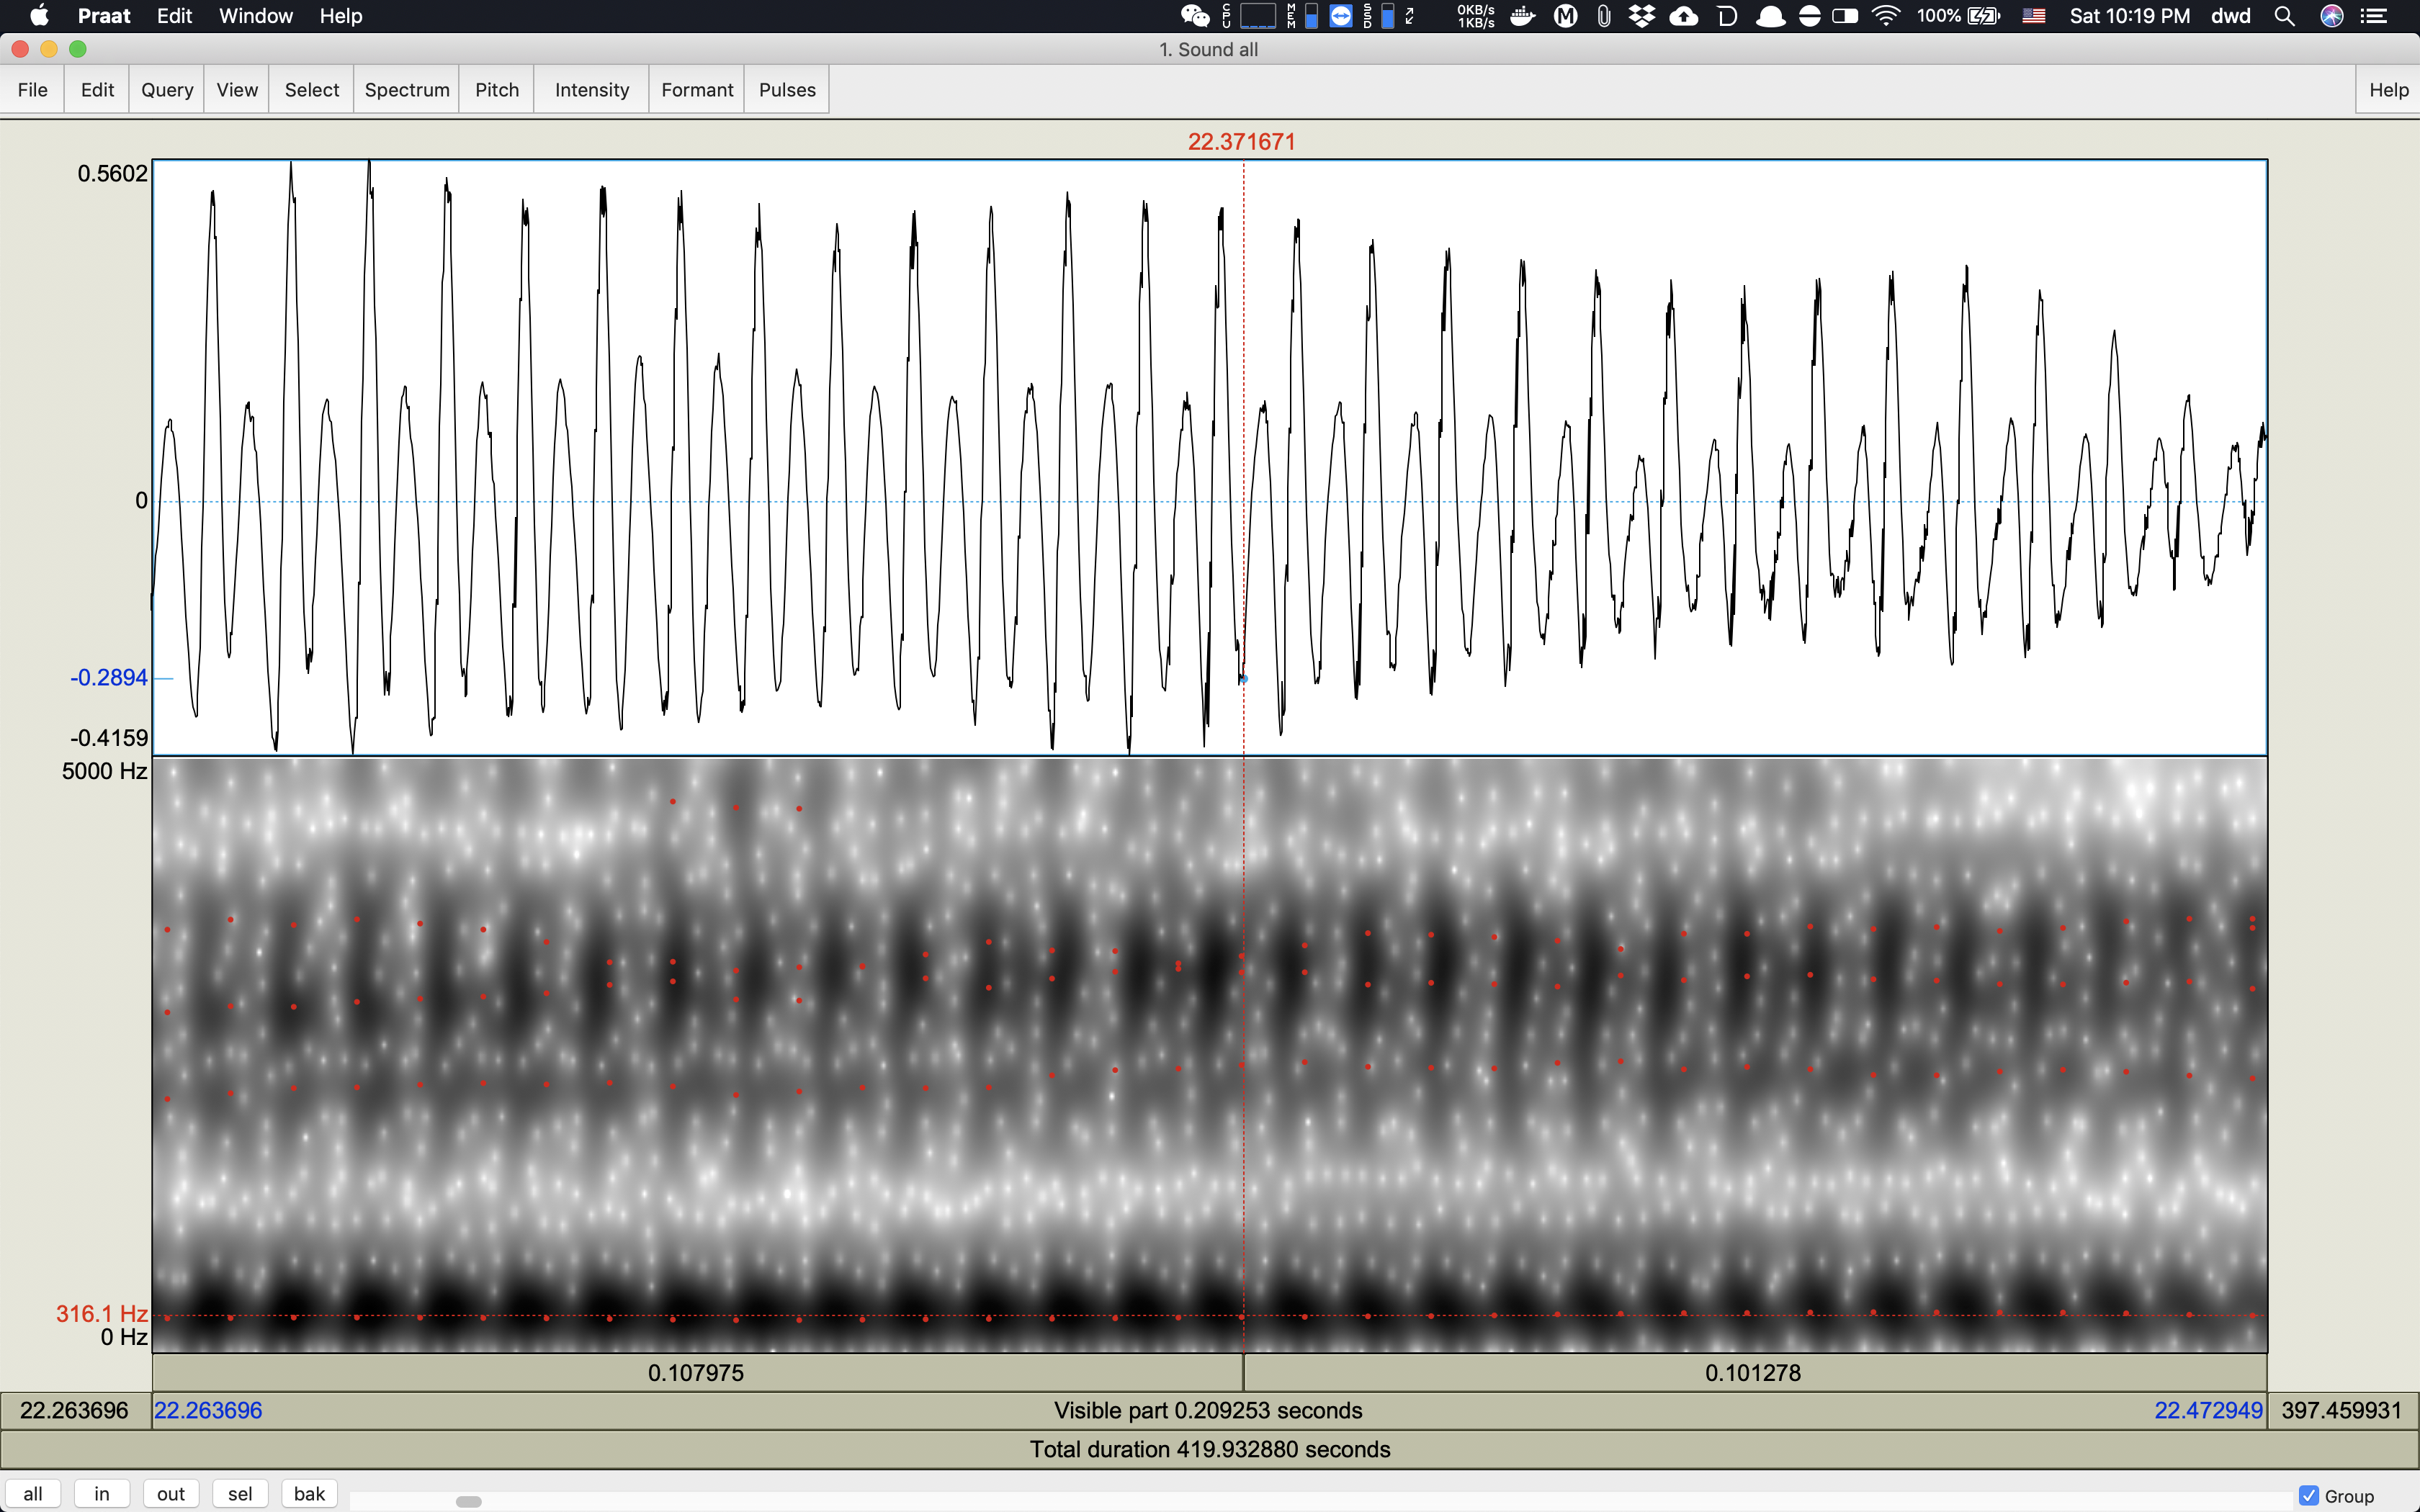
\includegraphics[scale=0.25]{imgs/vowel_i.png}
    \caption{[i]}
\end{figure}
\begin{figure}[H]
    \centering
    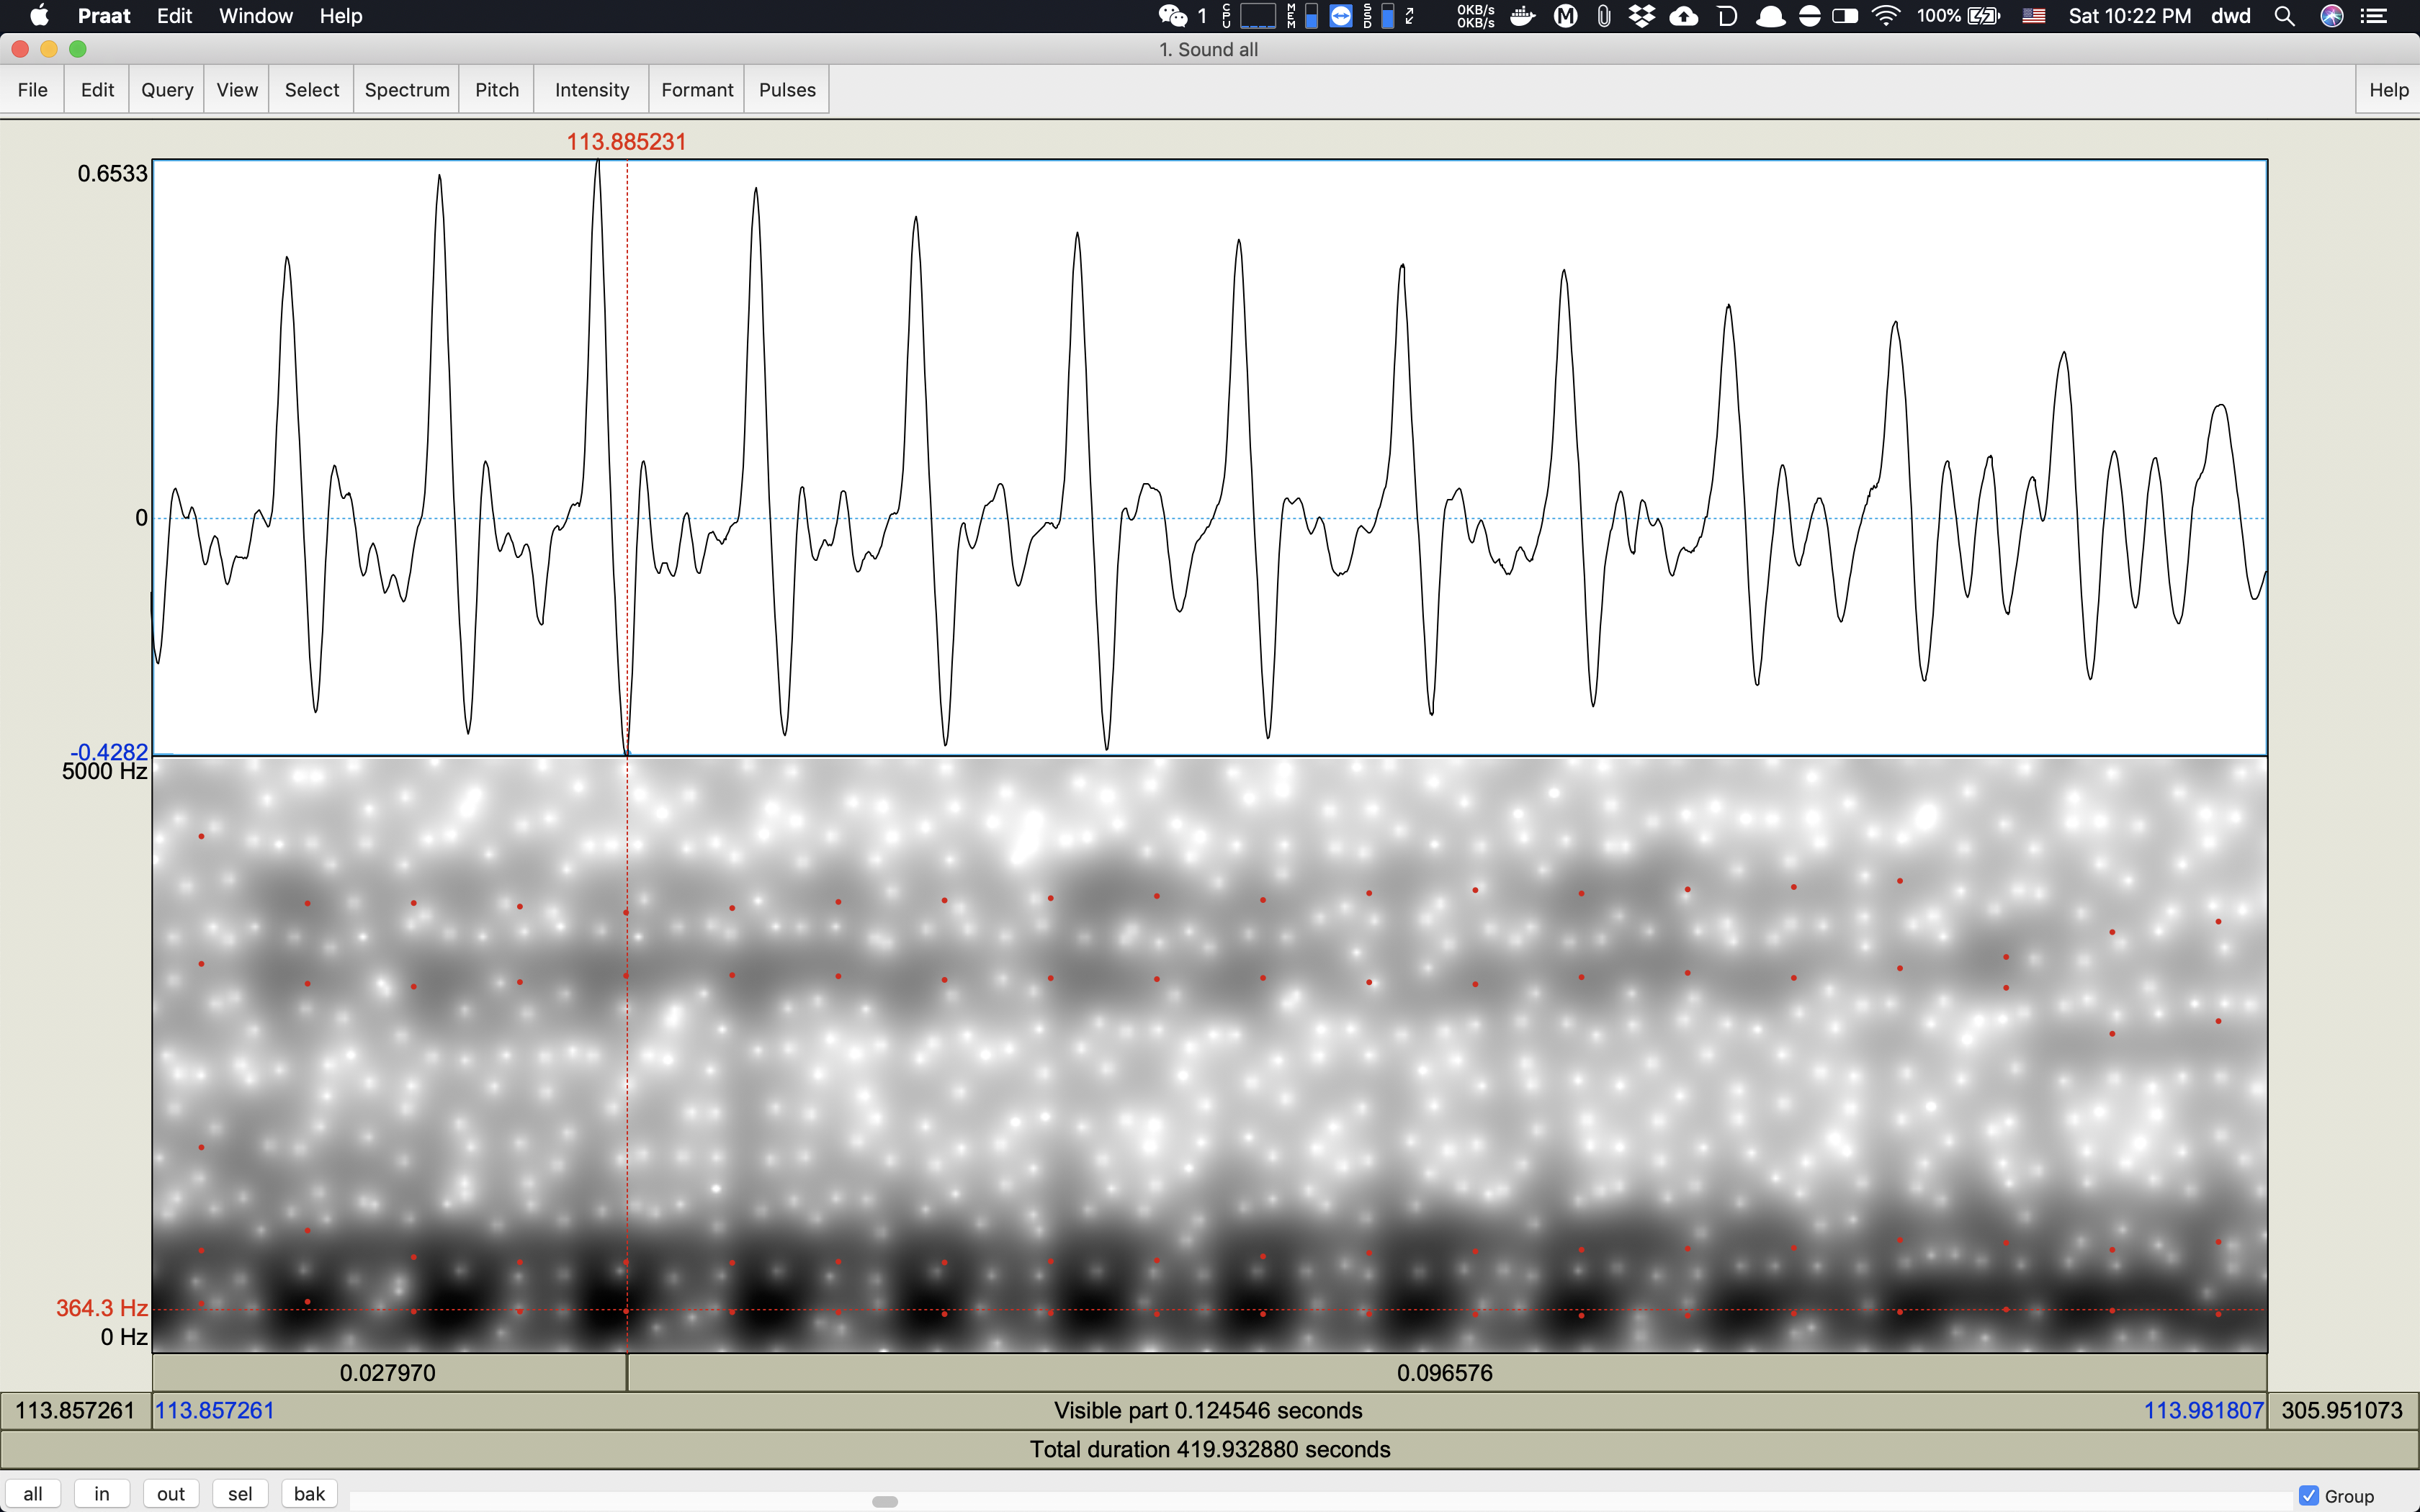
\includegraphics[scale=0.25]{imgs/vowel_u.png}
    \caption{[u]}
\end{figure}
\begin{figure}[H]
    \centering
    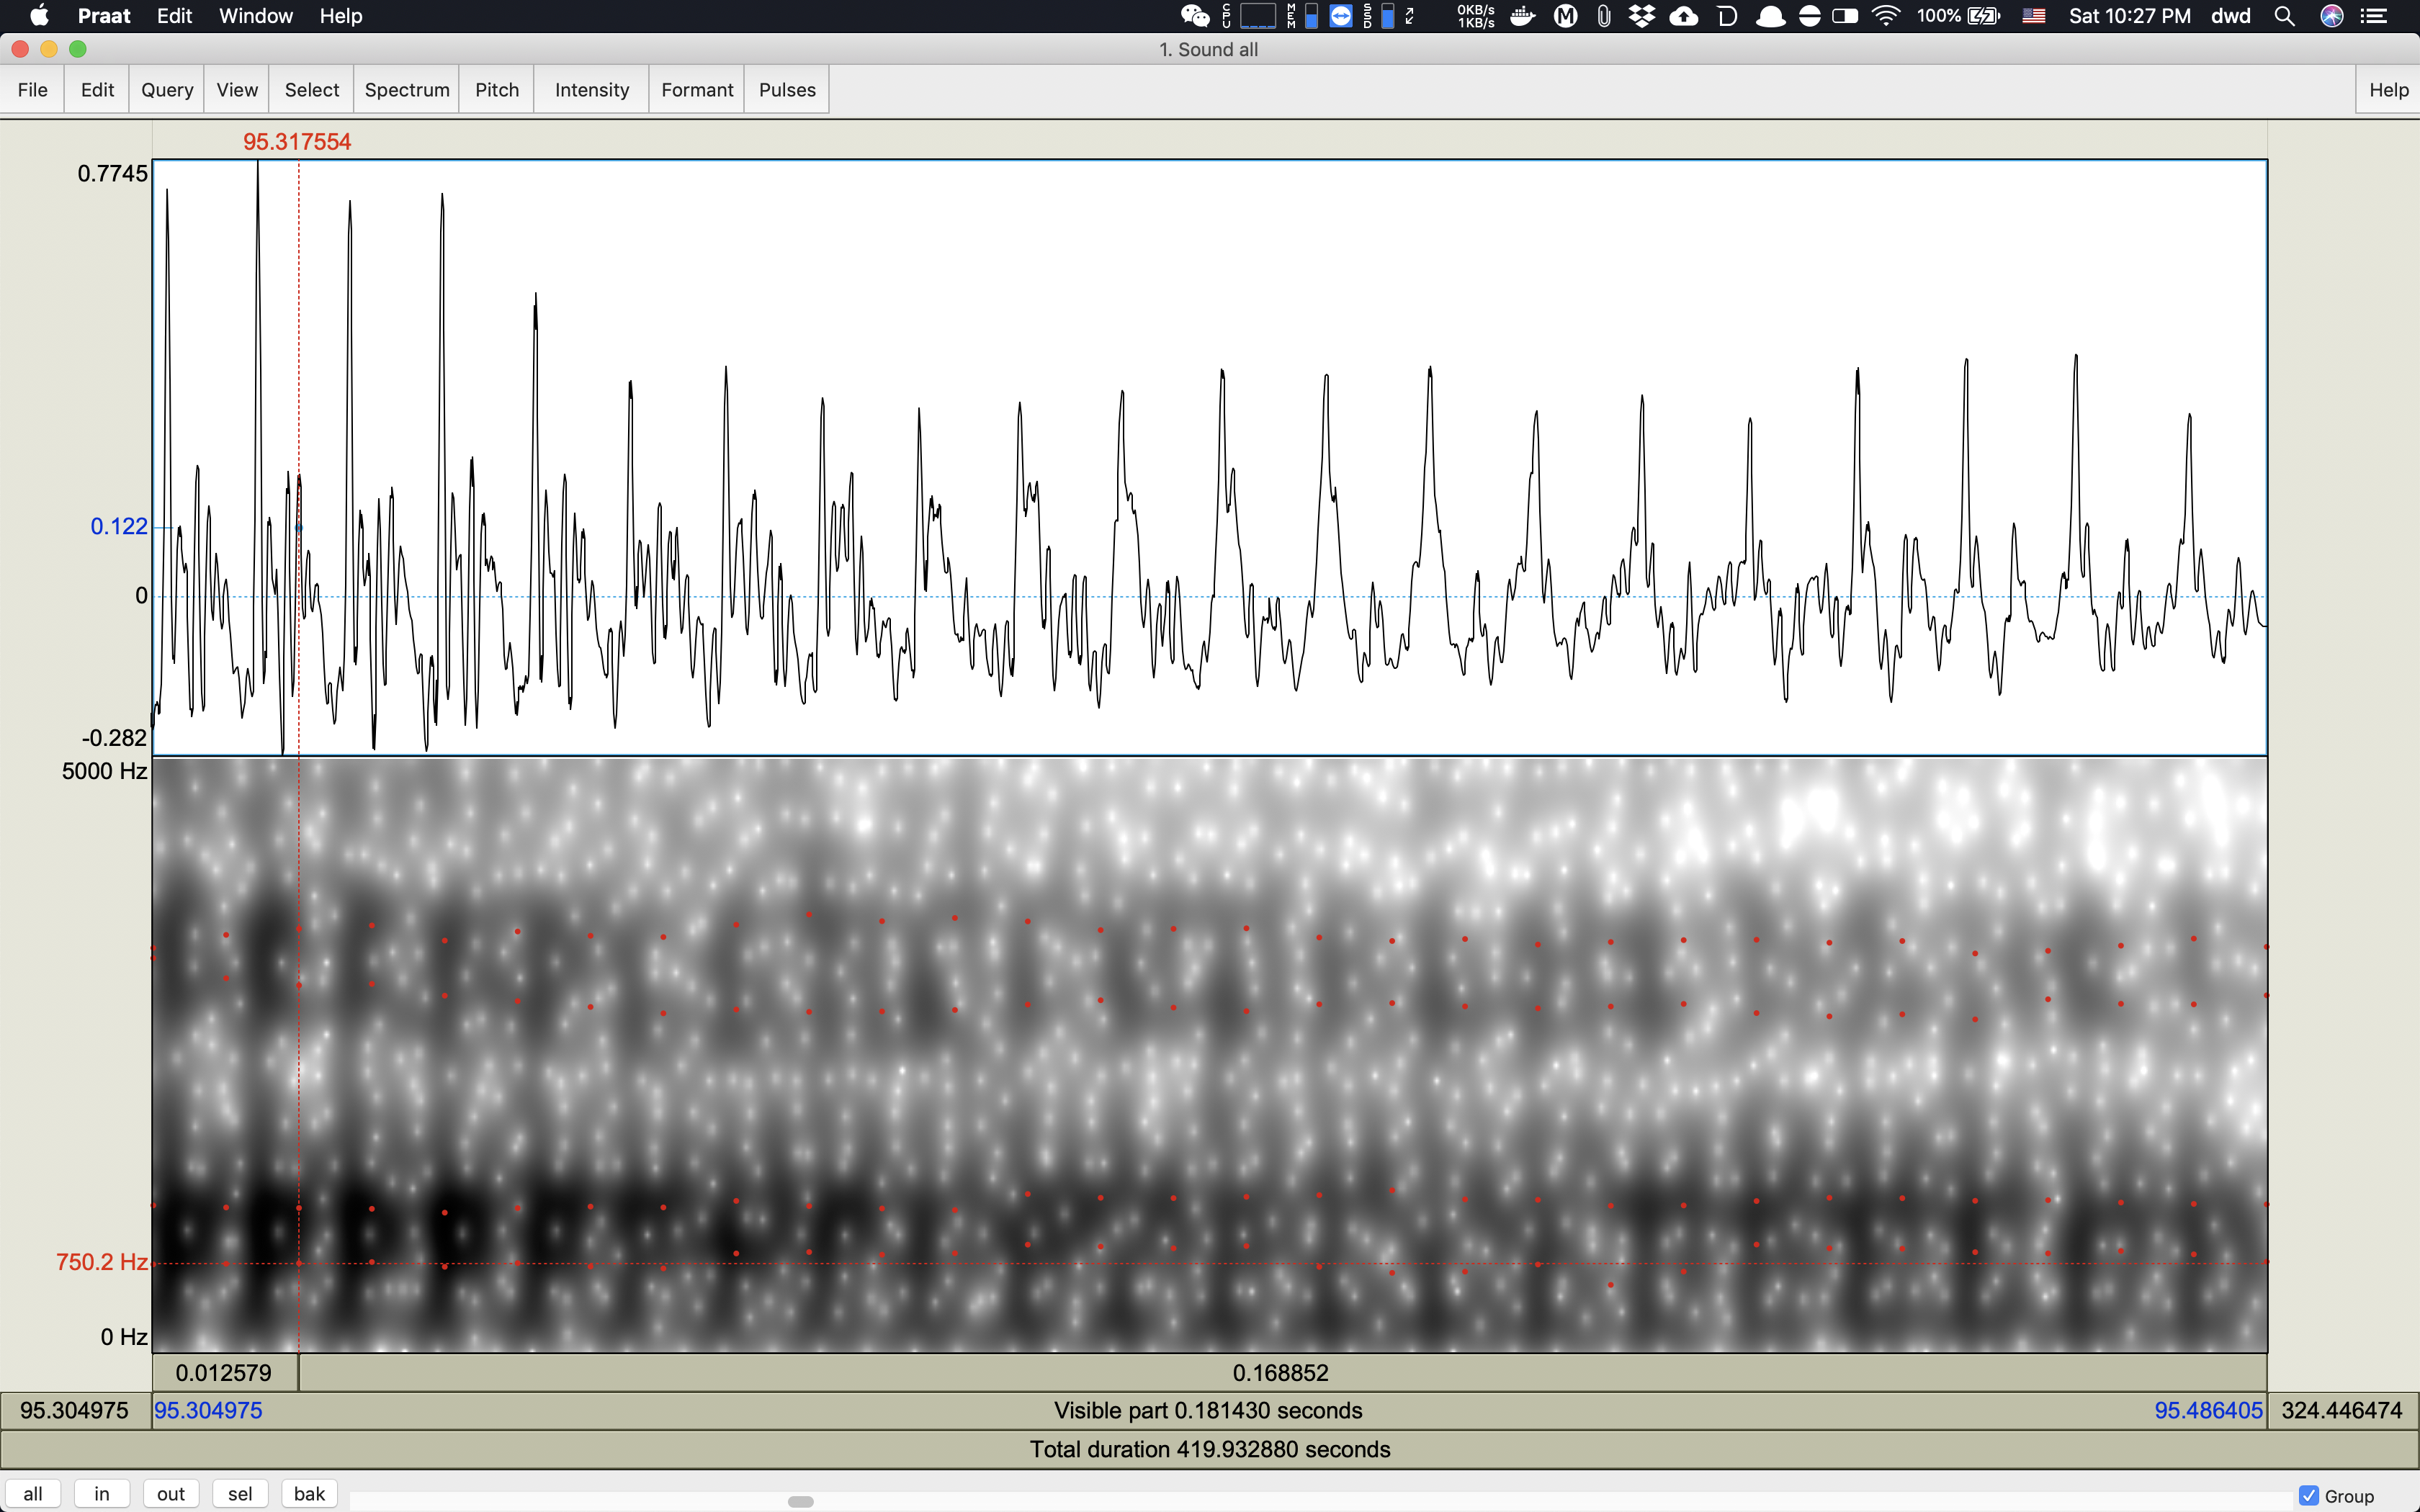
\includegraphics[scale=0.25]{imgs/vowel_a.png}
    \caption{[a]}
\end{figure}
\begin{figure}[H]
    \centering
    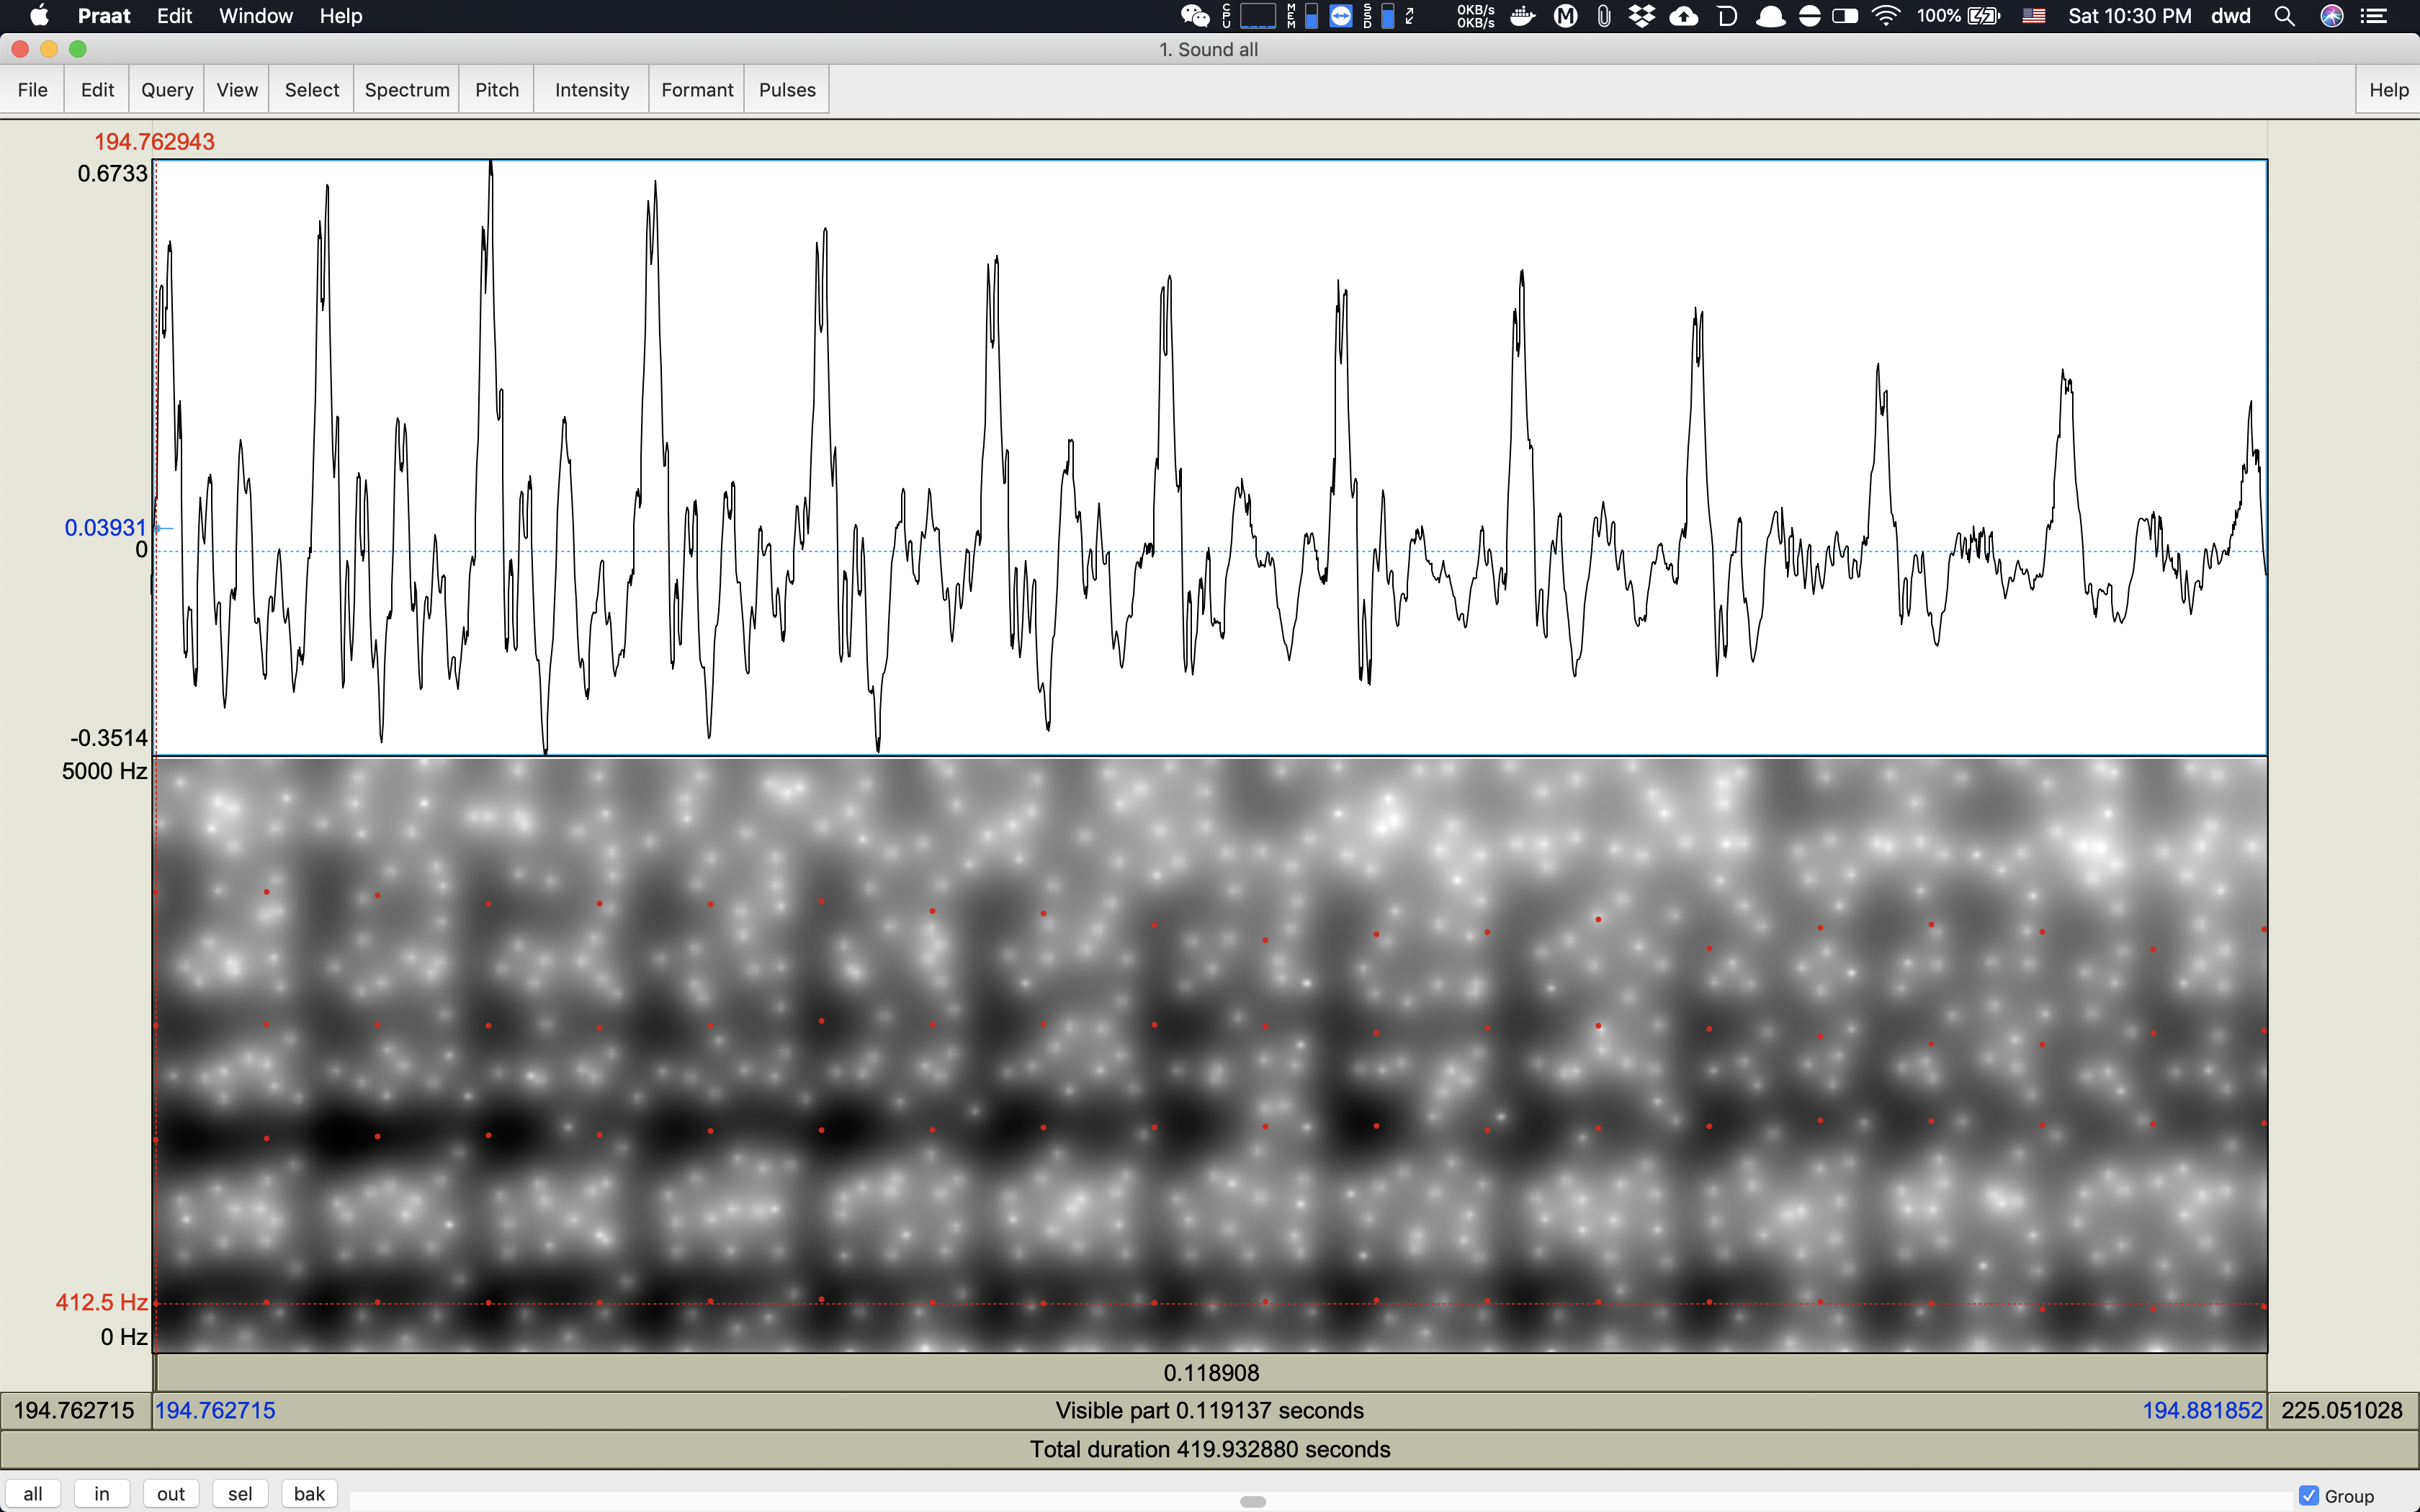
\includegraphics[scale=0.25]{imgs/vowel_e.png}
    \caption{[e]}
\end{figure}
\begin{figure}[H]
    \centering
    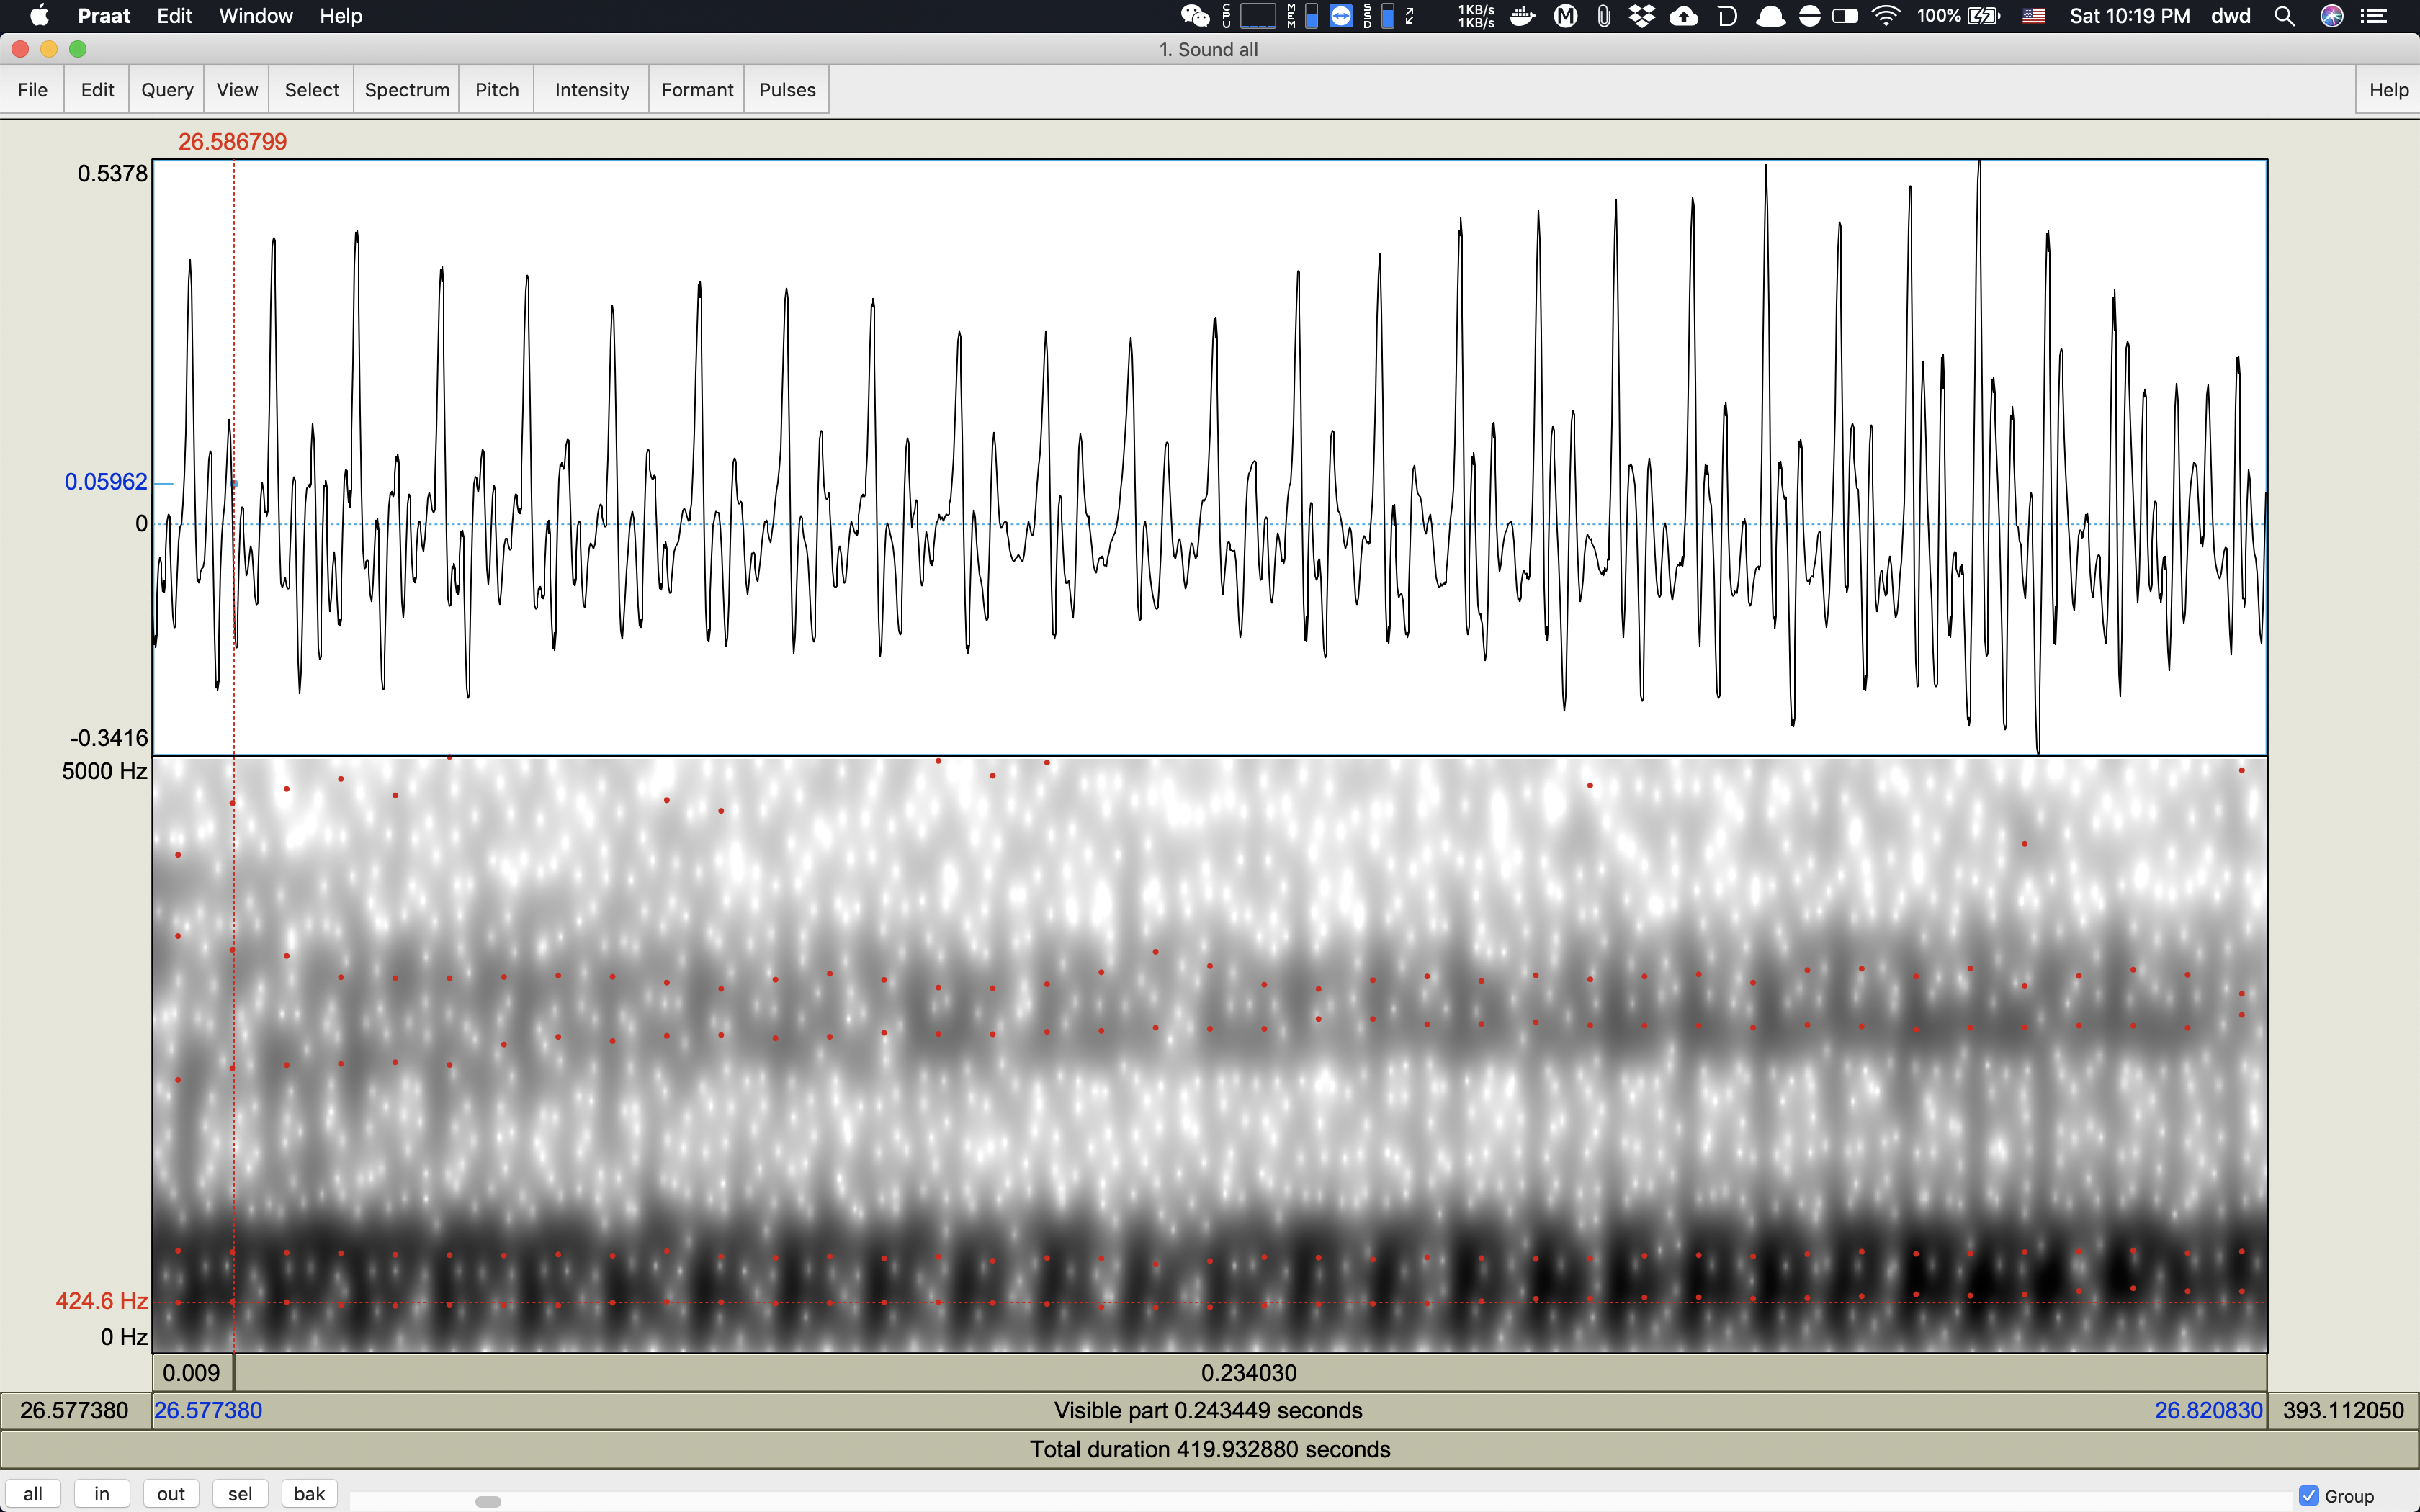
\includegraphics[scale=0.25]{imgs/vowel_o.png}
    \caption{[o]}
\end{figure}
\begin{figure}[H]
    \centering
    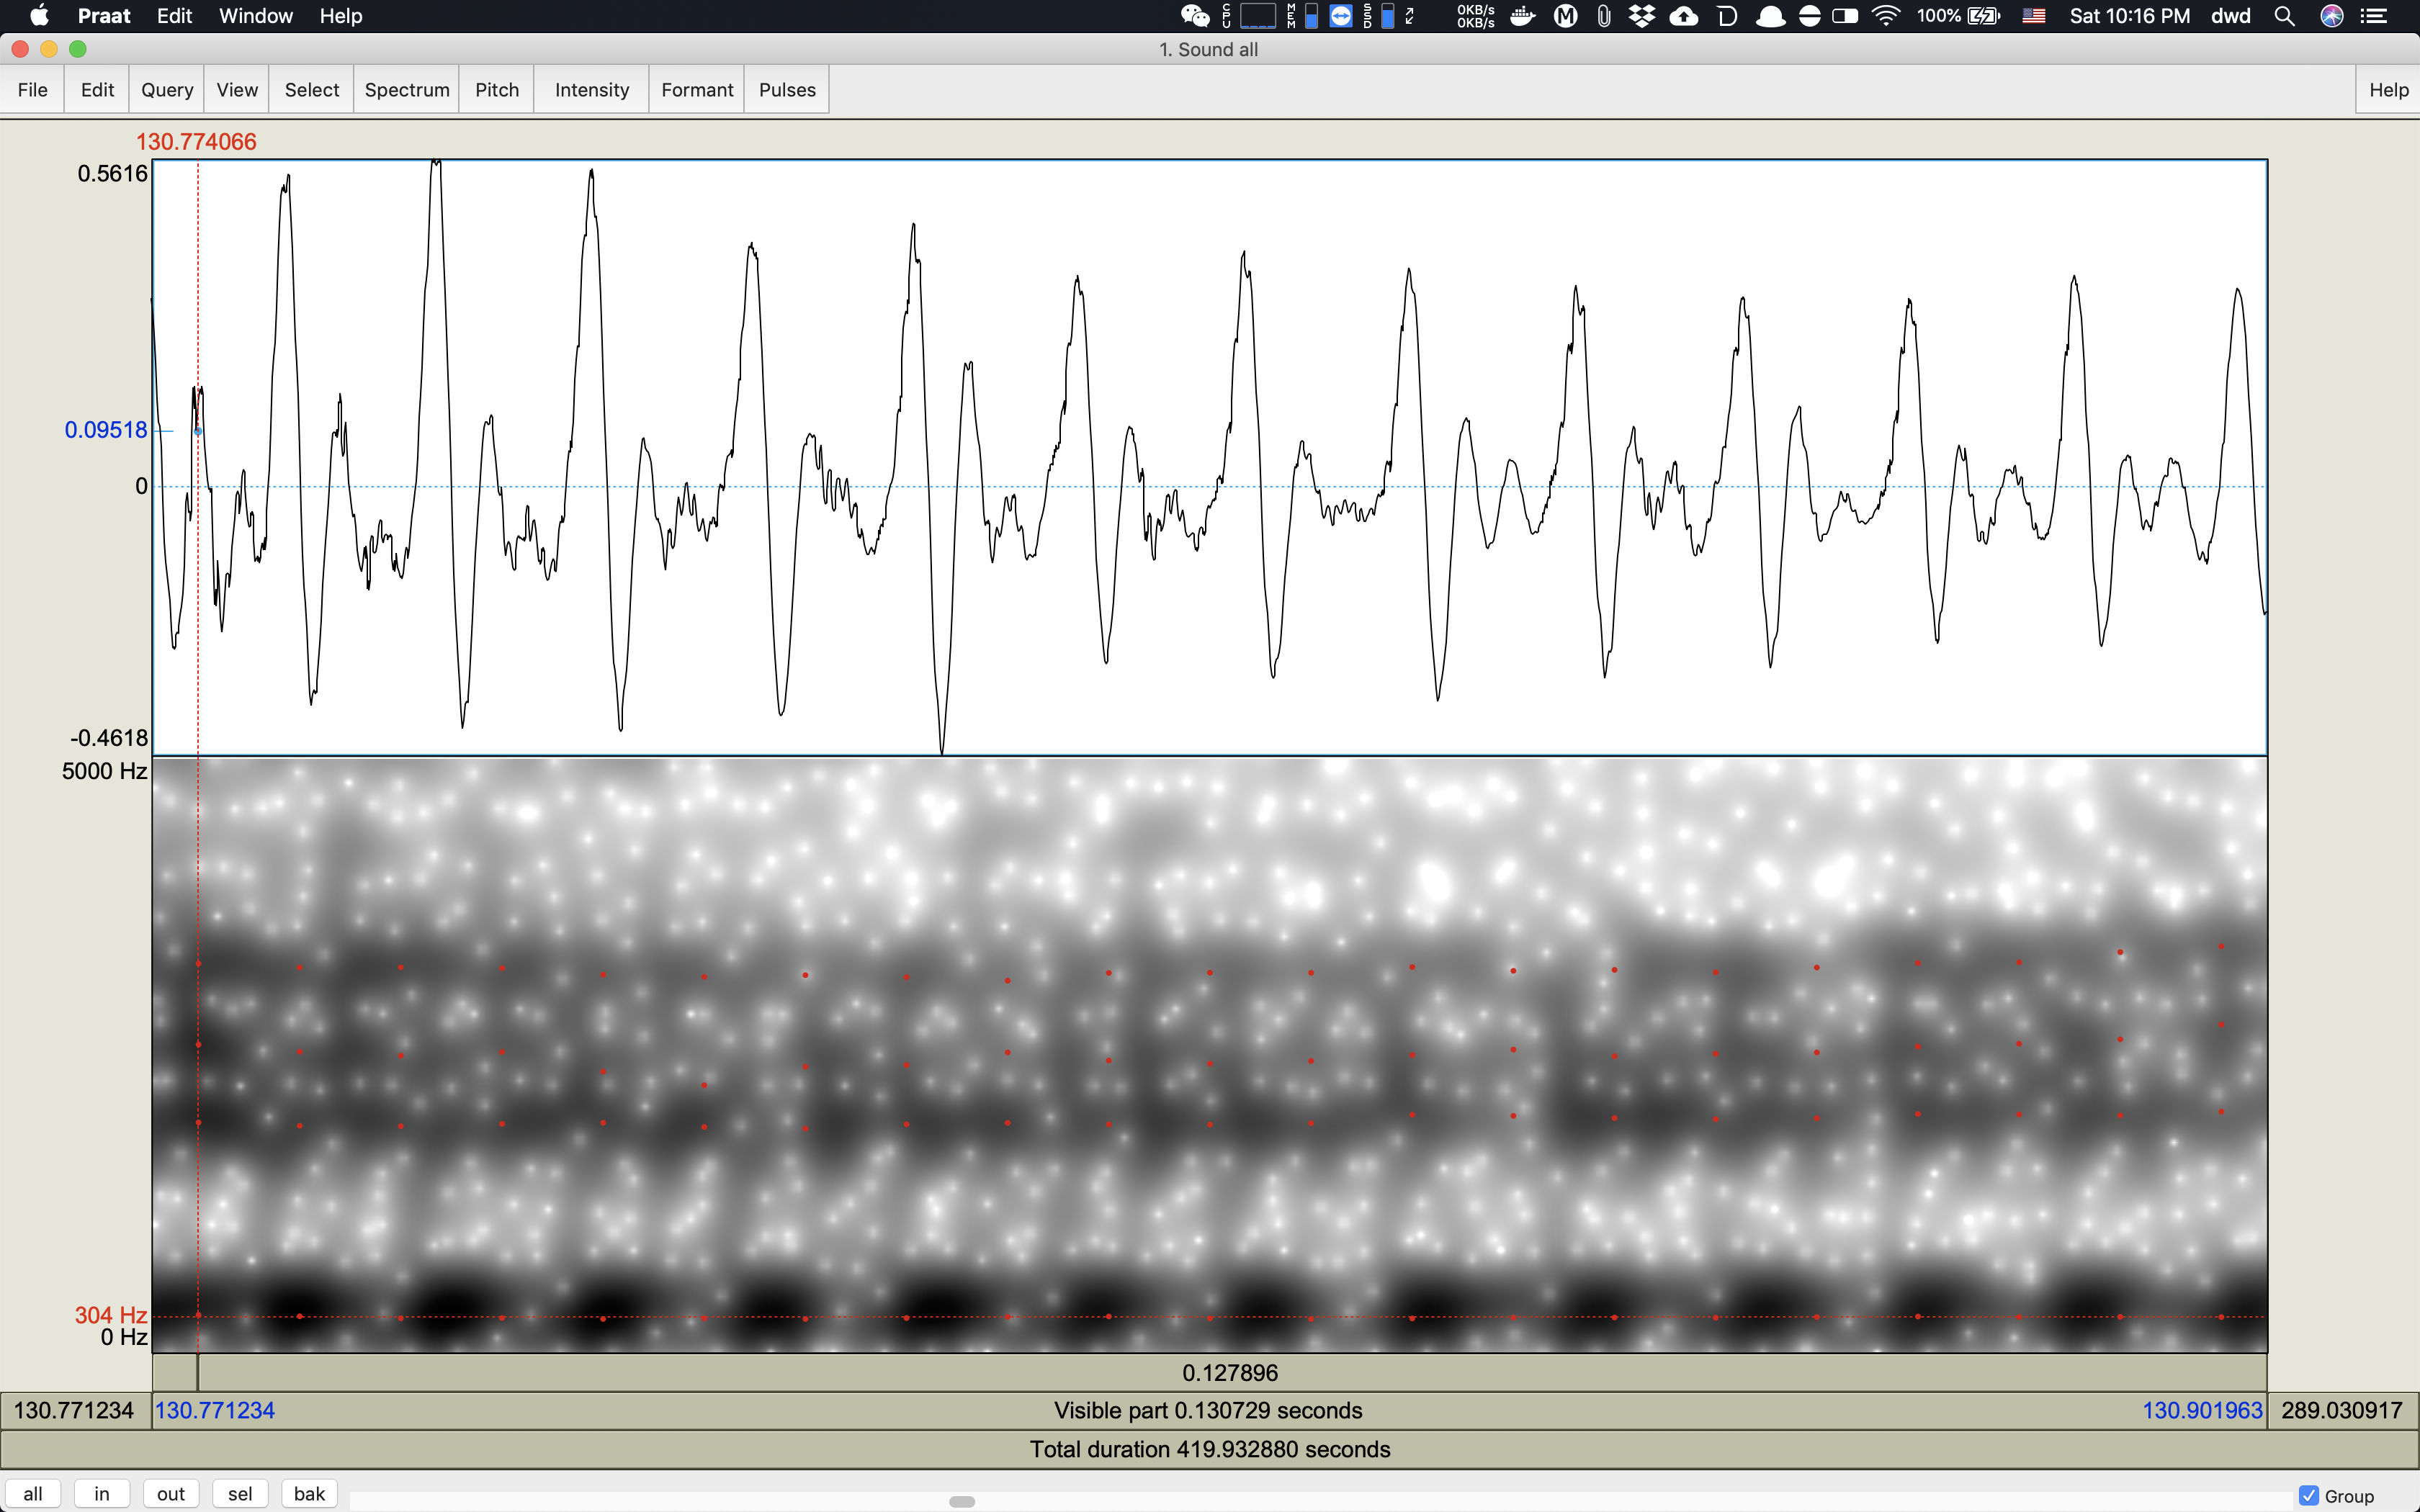
\includegraphics[scale=0.25]{imgs/vowel_y.png}
    \caption{[y]}
\end{figure}
\begin{figure}[H]
    \centering
    \includegraphics[scale=0.25]{imgs/vowel_œ.png}
    \caption{[œ]}
\end{figure}

\subsection{Vowel Space Plotting}
\begin{figure}[H]
    \centering
    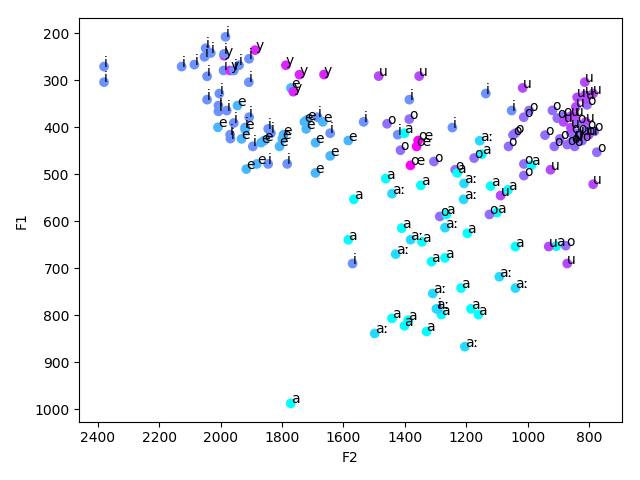
\includegraphics[scale=0.6]{imgs/vowelspace.png}
    \caption{vowel space of Cantonese (axes inverted)}
\end{figure}
The plotted vowel space bears some similarity with the vowel chart, at least the distribution of [i] (high and front), [a] (low and central), and [u] (high and back) is quite clear. Moreover, the location of [y] and [e] agrees well with their location in the vowel chart. Personally I think [u] and [o] are too close to each other, but it is still possible to see that [u] is higher than [o]. The position of [œ] is also quite ideal, though it appears to be more centralized than it should be. 

\subsection{Diphthong Movement}
\begin{figure}[H]
    \centering
    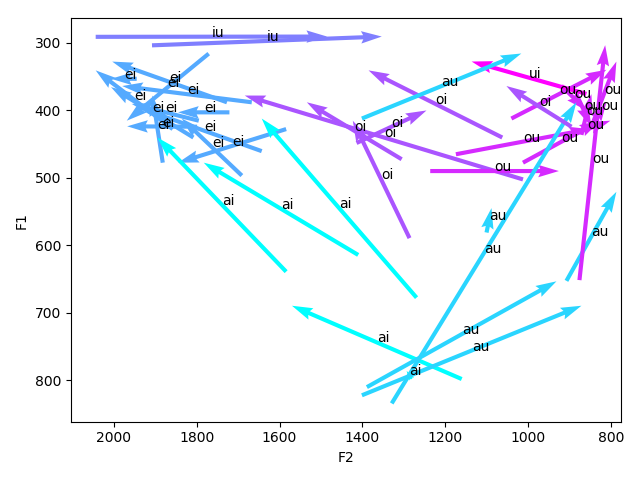
\includegraphics[scale=0.6]{imgs/diphthong_movement.png}
    \caption{diphthong movement of Cantonese (axes inverted)}
\end{figure}
The start of an arrow corresponds to the F1 and F2 value of the first phoneme in a diphthong, while the end of an arrow corresponds to that of the second phoneme. As we can see, the direction of arrows of a diphthong has a certain level of consistency.

\subsection{Vowel Variety and Symmetry}
According to the standard of WALS, Cantonese has a large vowel quality inventory (7 > 6). All vowels are peripheral. The vowel quality inventory is asymmetrical and the peripheral structure should be characterized as ``left'' since there are more front vowels than back vowels. 

\subsection{Vocal Tract Length Estimation}
This one is tough since there is no schwa in this small corpus. However, if we just try to eyeball the vowel space and figure out where a center might be, I think it should be somewhere around F1 = 450Hz, F2 = 1350Hz. As a result, $L = \frac{340}{4 * 450} = 0.189m = 18.9cm$, which looks reasonable for a 23-year-old human male with a height of 1.8m.


\section{Tone System}

\subsection{Overview}
Cantonese has 6 lexical tones. There may be some sources online claiming that there are 9 tones. However, the extra three are the so-called ``entering tones'', marking unusual unvoiced consonant codas like [p], [t], and [k] that are rare in Sinitic languages. In this small corpus a few [\textglotstop] can be observed, which arguably come from [t]. There is a very audible [p], in the $95^{th}$ word [kap]. In the $93^{th}$ word there is also a well-heard [sik]. In conclusion, whether there are nine tones or six tones is more of a matter of regional pride that linguistics. I'll stick to the six-tone version in the following discussion since this definition of tone has more to do with acoustics.

\subsection{Caveat}
When I was doing Milestone 3, I had the feeling that the acoustic measurement of f0 on the vowel does not always agree with auditory impression. I later found out that this inconsistency is largely caused by sonorant onsets and codas. For instance, for a syllable with nasal coda that has a perceivably rising tone, the rising part may actually happen in the nasal coda. This suggests that tone, as an acoustic feature, should be considered on the syllabic level. 

As a result, doing clustering analysis over the vowel f0 may end up giving more false discoveries than true insights. This saddens me for a brief moment. Anyway, I'll try to talk about examples of the six tones in the following sections, hoping that they can bear some scientific weights. 

\subsection{Tones}

\subsubsection{Tone(55): High and Flat}
This is probably the most distinguishable tone. Its f0 contour is extremely flat at the level from 110Hz to 130Hz (which is already the highest for my speaker in normal speech). It is the same as the first tone of Mandarin. 

The following figure is the waveform and spectrogram for [i] in [bin55], which means ``what''. f0 is flat at 117Hz. 
\begin{figure}[H]
    \centering
    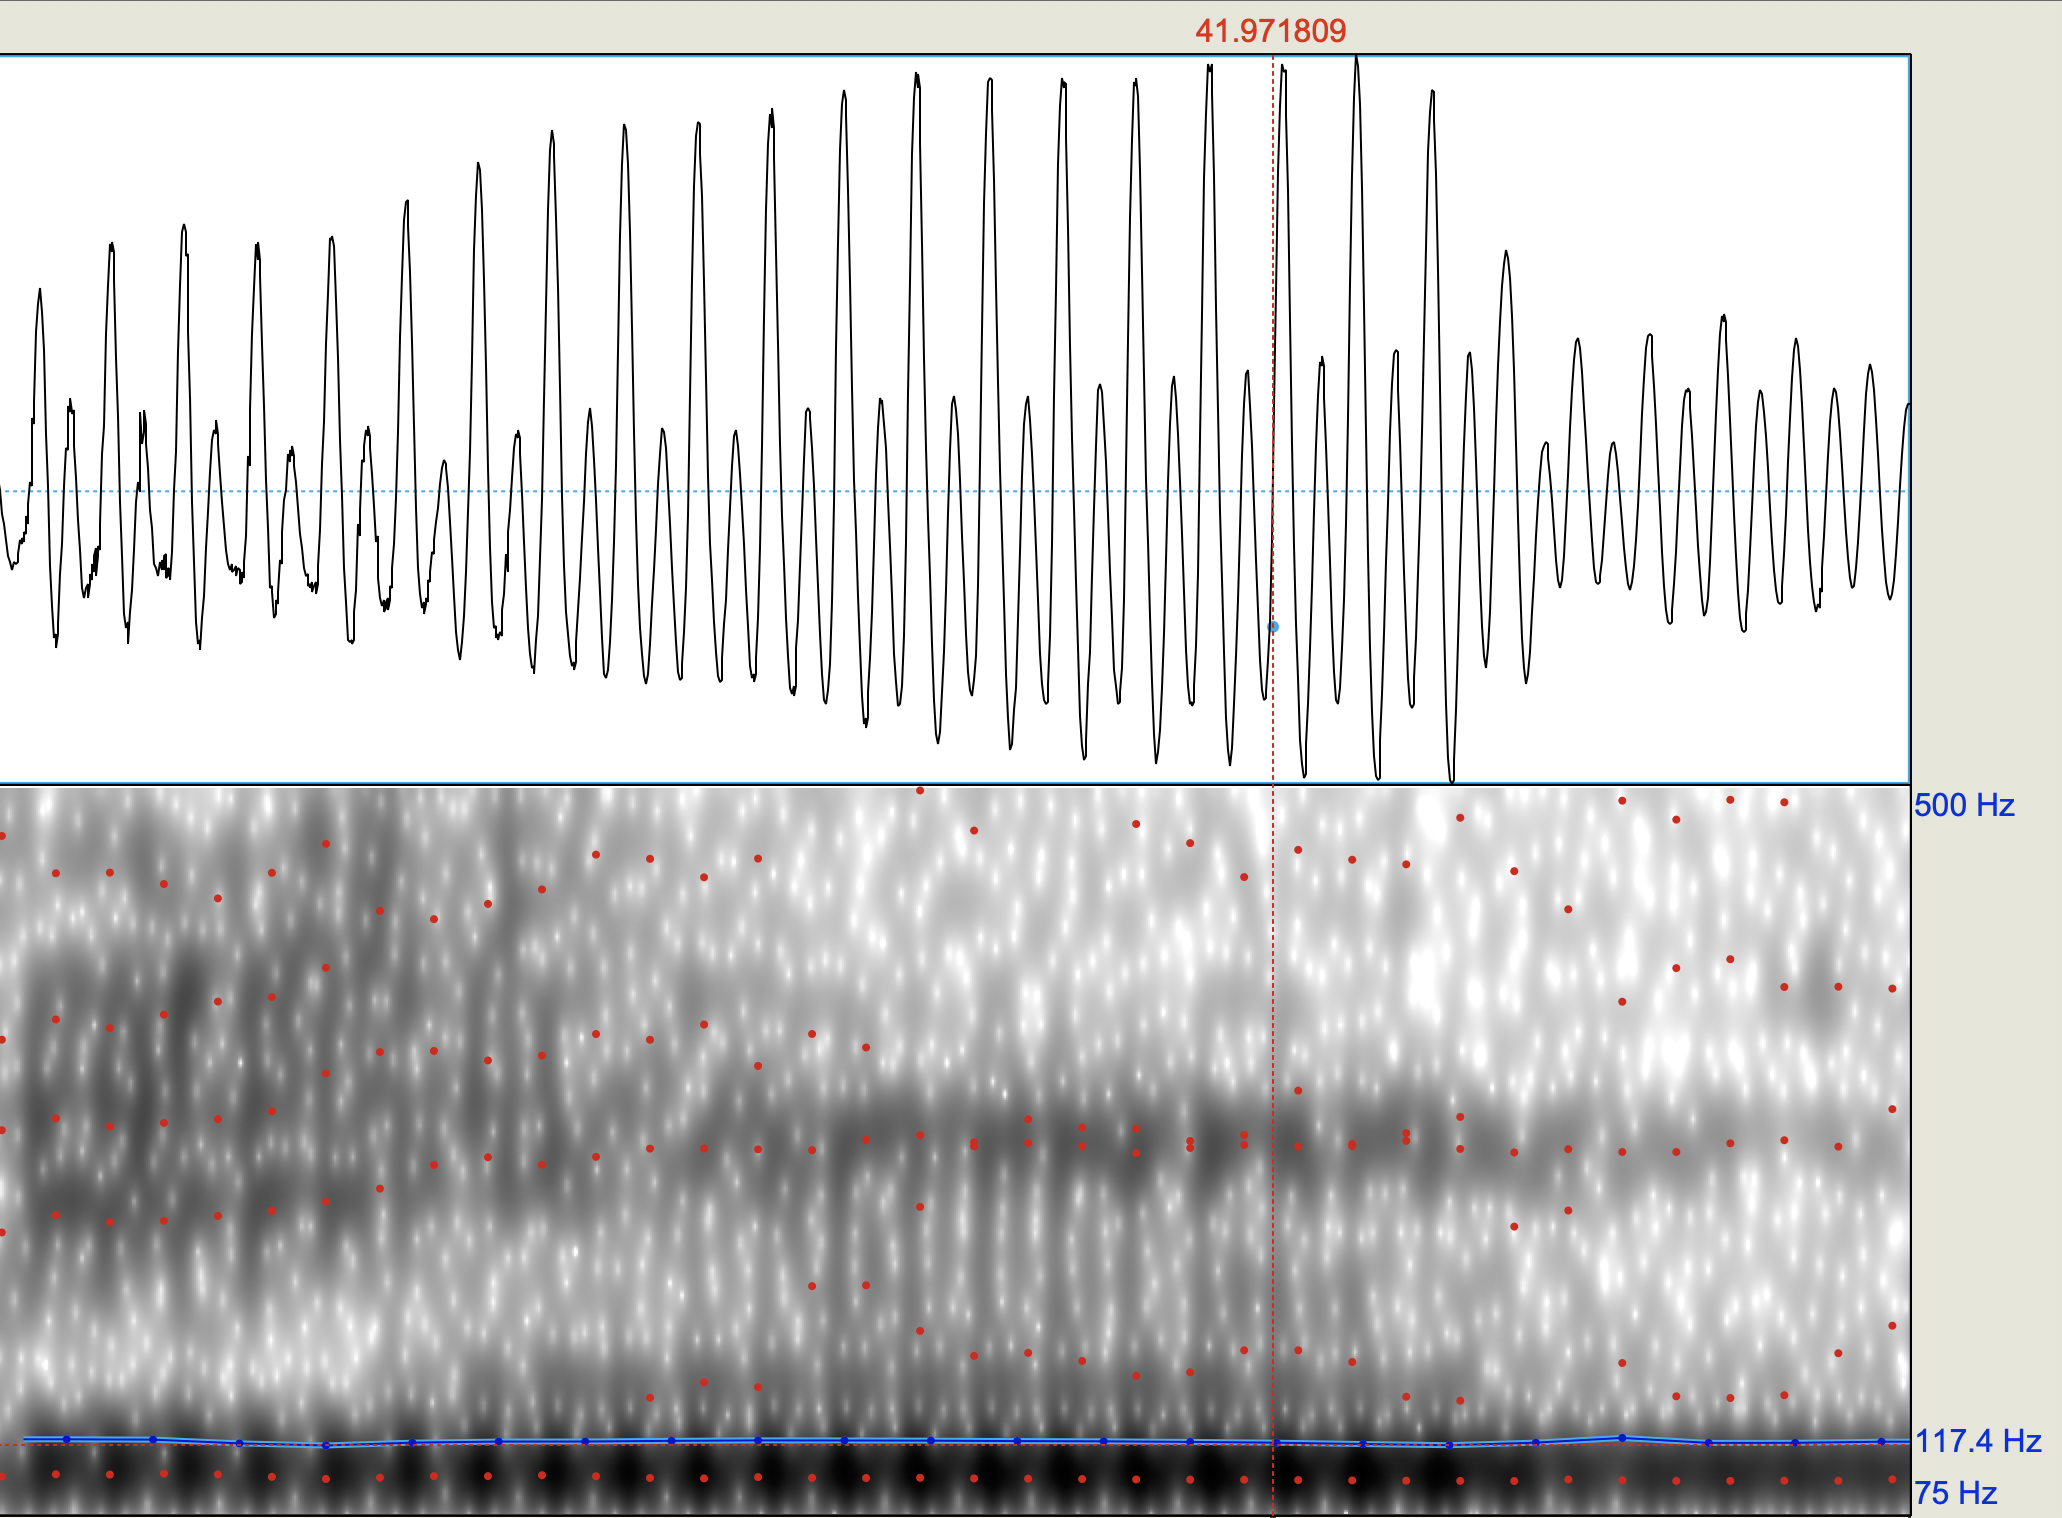
\includegraphics[scale=0.4]{imgs/tone55.png}
    \caption{Tone(55): High and Flat}
\end{figure}

\subsubsection{Tone(325): Mid and Rising}
This sounds like something followed by a question mark. Its f0 contour usually has a small drop in the beginning, going from around 105Hz to below 100Hz. Then a long and audible rise goes from there all the way to the level of the High Flat tone. It is the same as the second tone in Mandarin.

The following figure is the waveform and spectrogram for [i] in [si325], which means ``history''. 
\begin{figure}[H]
    \centering
    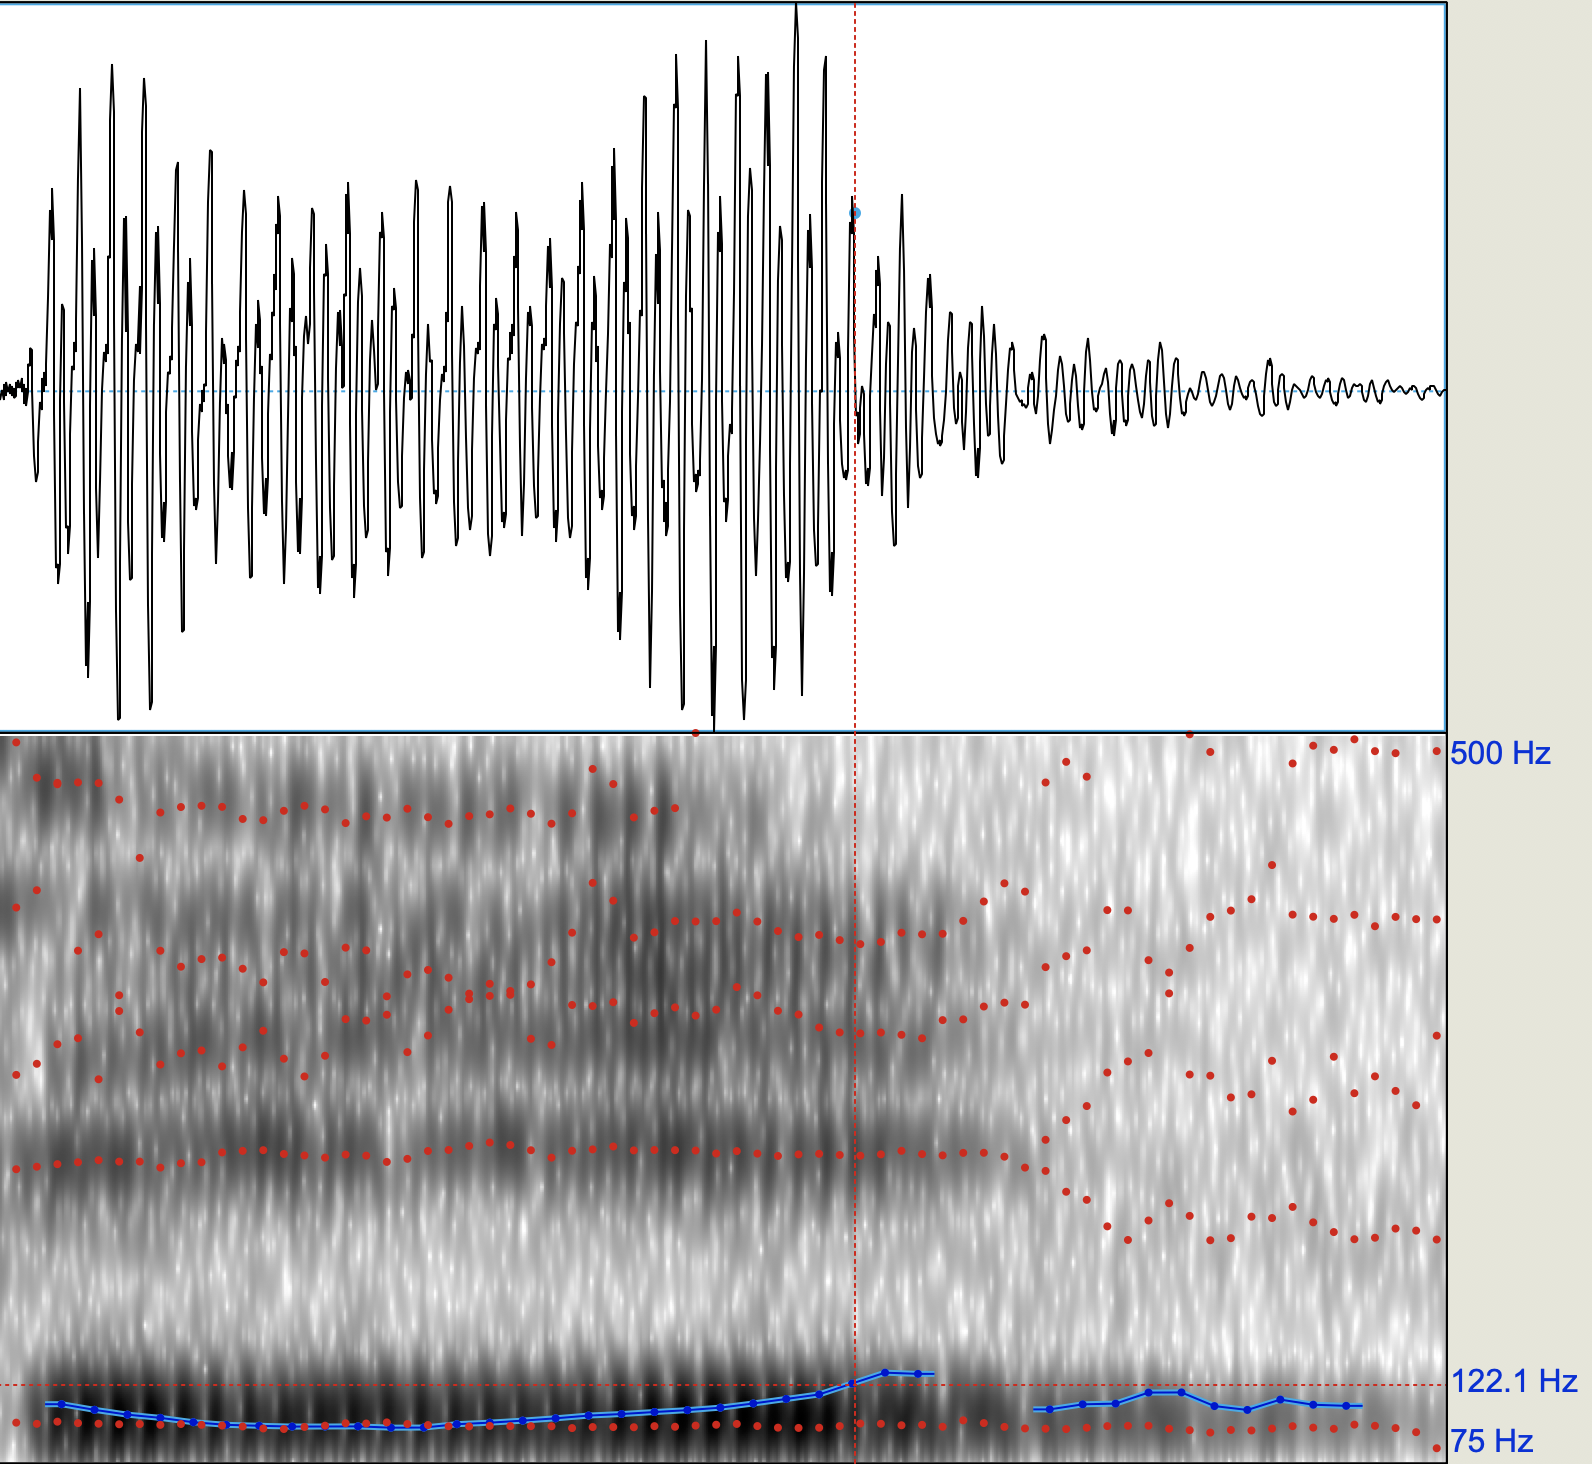
\includegraphics[scale=0.4]{imgs/tone325.png}
    \caption{Tone(325): Mid and Rising}
\end{figure}

\subsubsection{Tone(33): Mid and Flat}
In terms of auditory experience, it is easy for a native speaker of Beijing dialect to confuse it with the "first tone". However, this tone tends to be flat at a lower level, typically somewhere between 100Hz and 105Hz. This tone is not present in Mandarin. 

The following figure is the waveform and spectrogram for [i] in [si33], which means ``try''. 
\begin{figure}[H]
    \centering
    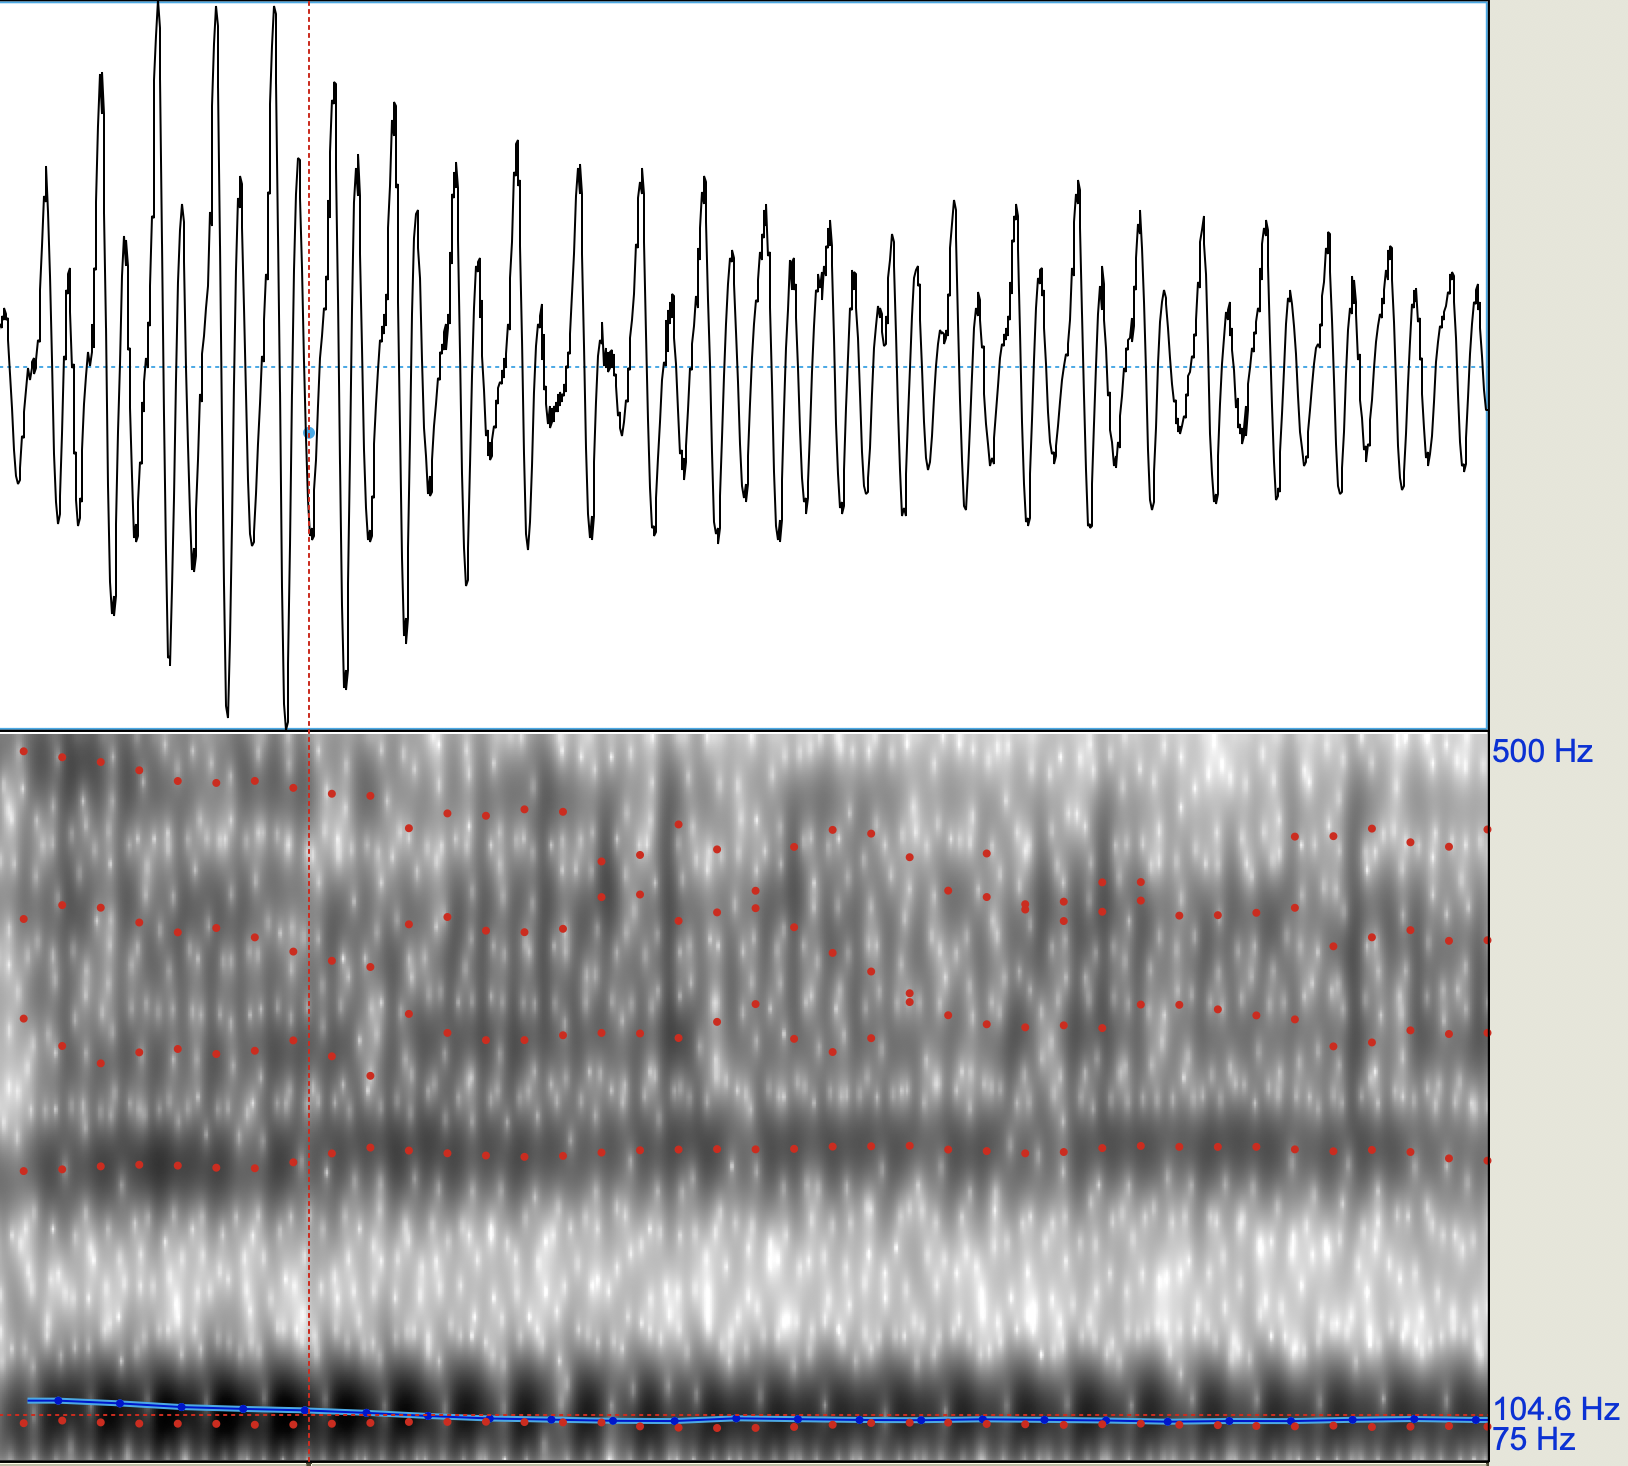
\includegraphics[scale=0.4]{imgs/tone33.png}
    \caption{Tone(33): Mid and Flat}
\end{figure}

\subsubsection{Tone(21): Low and Falling}
In terms of auditory impression, this sounds like the third tone in Mandarin. Empirically speaking, this tone tends to shorten voicing, although more data is needed for validation. 

The following figure is the waveform and spectrogram for [jan21], which means ``man(human)''. 
\begin{figure}[H]
    \centering
    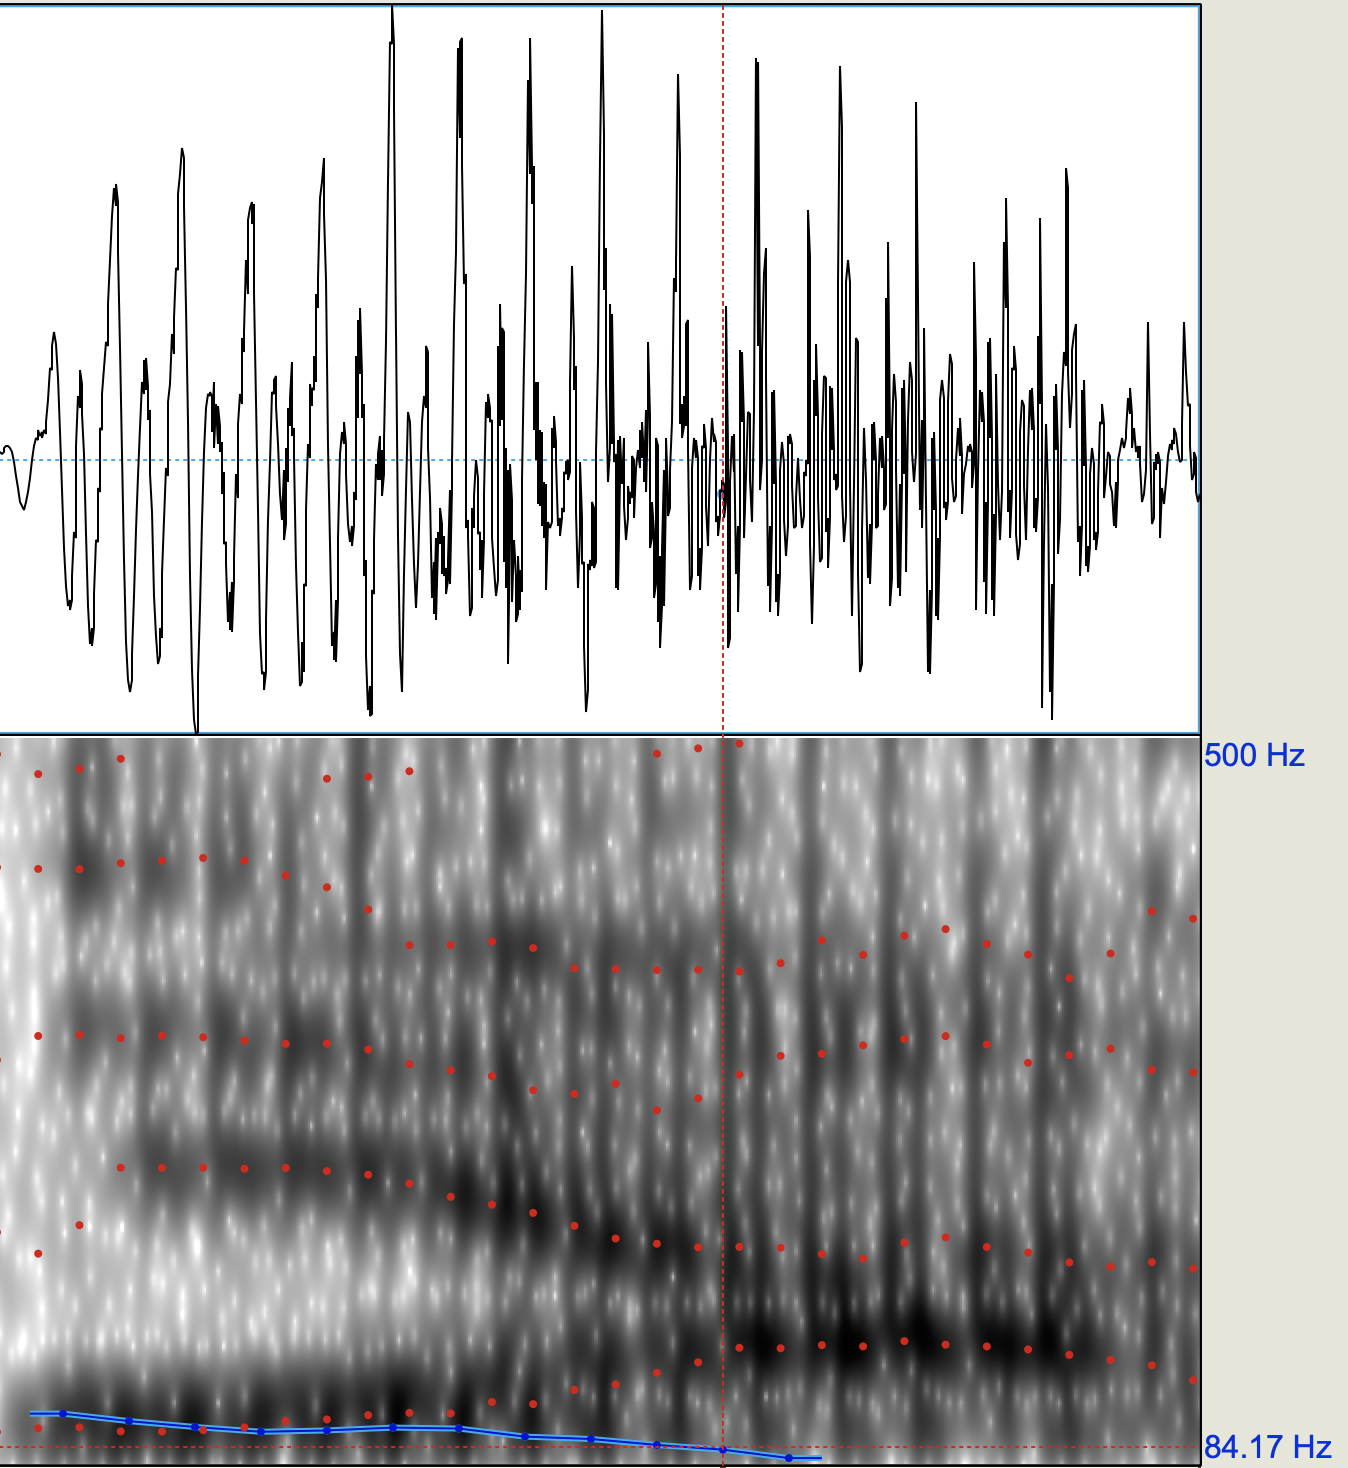
\includegraphics[scale=0.4]{imgs/tone21.png}
    \caption{Tone(21): Low and Falling}
\end{figure}

\subsubsection{Tone(23): Low and Rising}
It is easy for a speaker of Mandarin to confuse it with a tempered version of the ``second tone''. However, it sounds much lower across the f0 contour, typically from 90Hz to 110Hz. 

The following figure is the waveform and spectrogram for [i] in [si23], which means ``city/market''.
\begin{figure}[H]
    \centering
    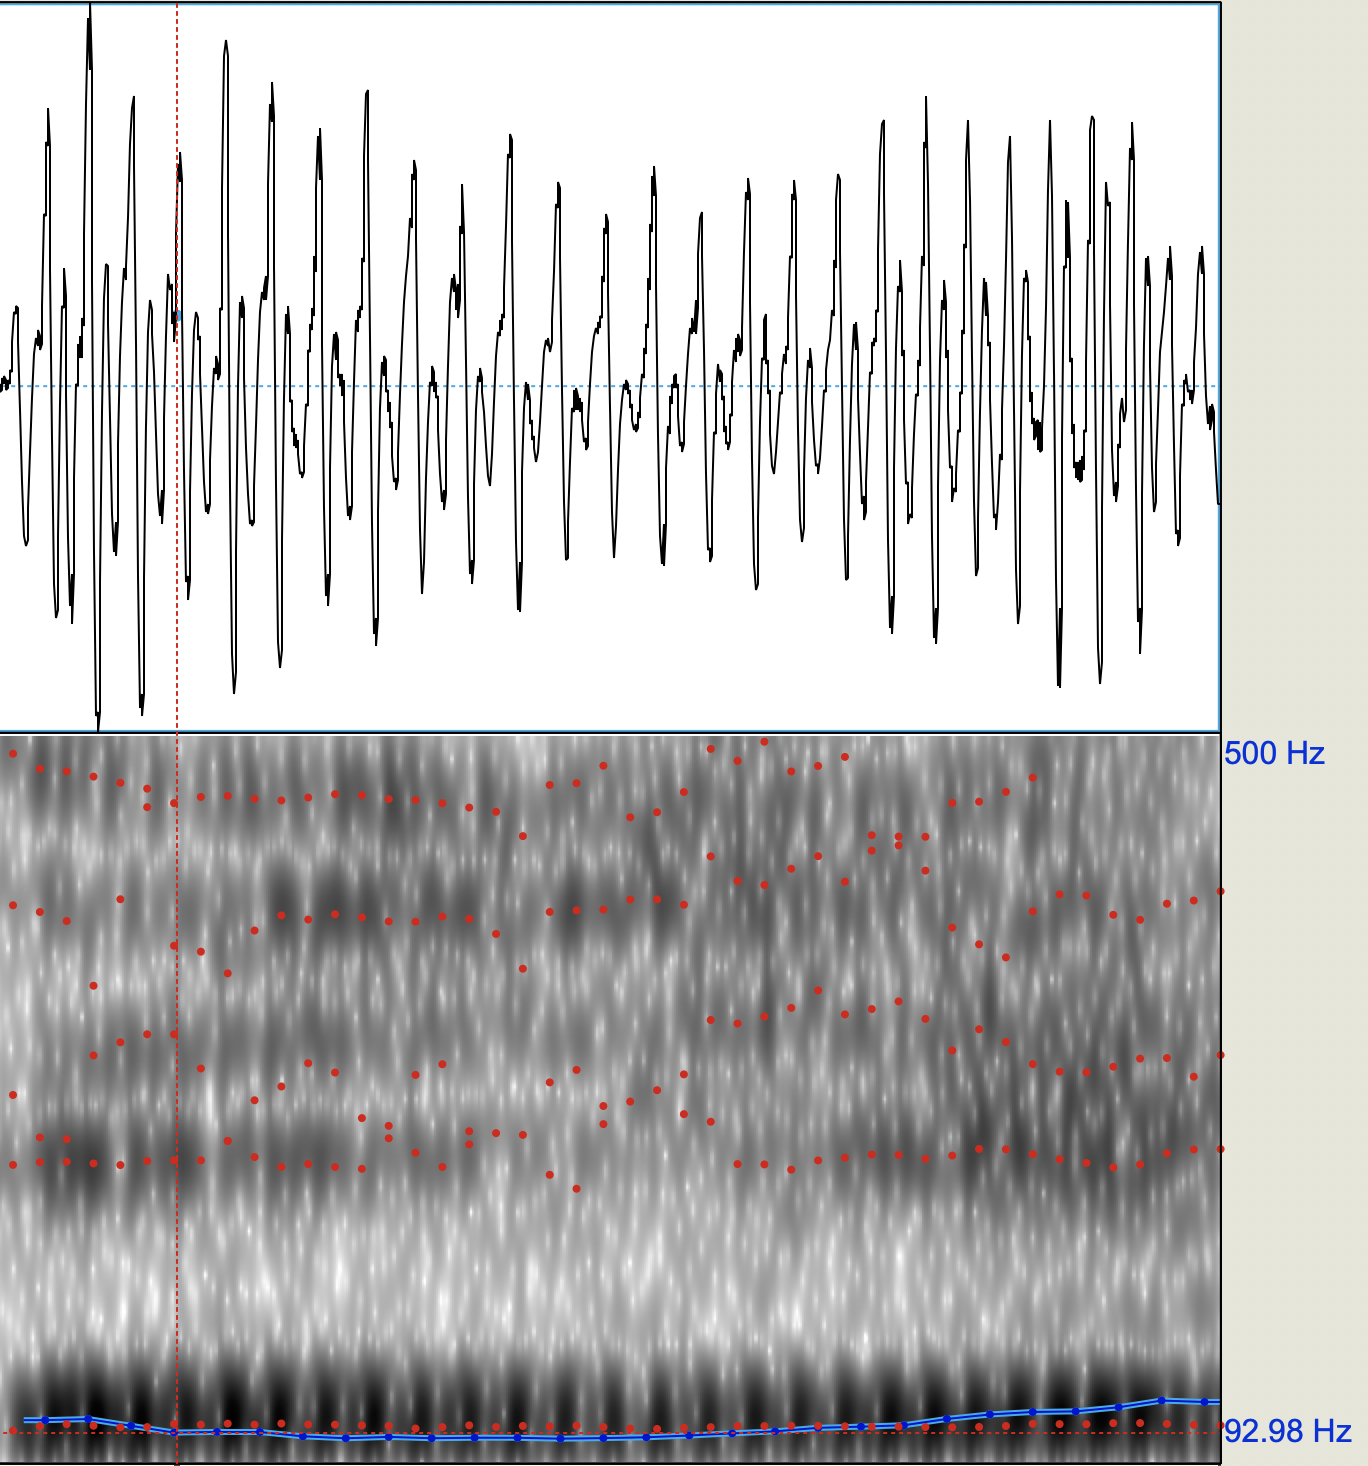
\includegraphics[scale=0.4]{imgs/tone23.png}
    \caption{Tone(23): Low and Rising}
\end{figure}

\subsubsection{Tone(22): Low and Flat}
During the articulation of a syllable of tone22, the speaker can hold the tone flat at around 90Hz for quite a while. This is a short drop in the beginning of voicing, but it is not as drastic as the Low Falling tone. 

The following figure is the waveform and spectrogram for [jan22], which means ``blade(knife)''.
\begin{figure}[H]
    \centering
    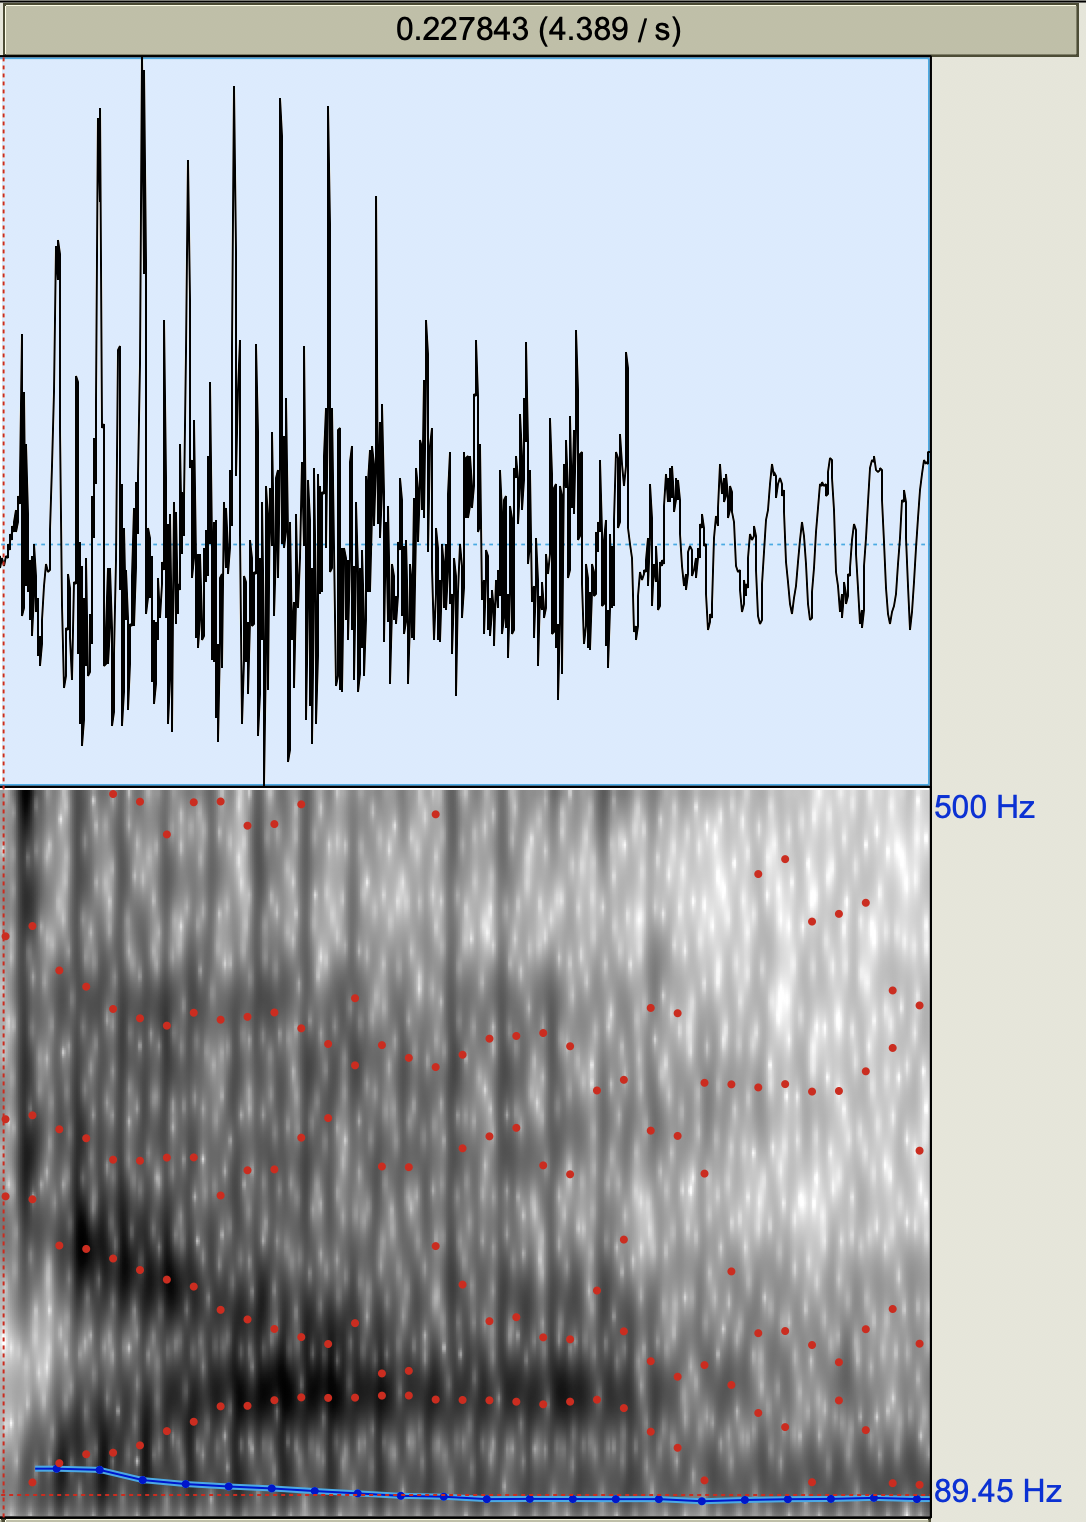
\includegraphics[scale=0.4]{imgs/tone22.png}
    \caption{Tone(22): Low and Flat}
\end{figure}

\subsection{Discussion}
Analyzing the tones only makes me more confused about speech perception. As we can see, the difference between the High Flat tone and the Mid Flat tone is largely about different levels of fundamental frequency. Since fundamental frequency is tightly related to speaker identity and humans have the ability to understand the same sentence spoken by different speakers, I think the following spectculations may be valid:

\begin{itemize}
    \item When hearing sentence spoken by an unknown speaker, we probably don't process input audio in a one-pass fashion, since if we don't have a clear idea about the "usual pitch" of this particular speaker and we don't keep memory of what has been heard from him/her, we won't be able to figure out which are tone(33) and which are tone(55). 
    \item Our perception of speech is tied with speaker identity. The Mid Flat tone(or even Low Flat tone) of a female speaker might be way higher than the High Flat tone of a male speaker. However, if both are familiar speakers, a person should have no difficulty telling the tones apart. This is in accordance with the Exemplar theory of speech perception. 
\end{itemize}

You might have noticed that the fourth tone of Mandarin(51, High-Falling tone) is absent in Cantonese. That's only because we haven't seen a proper context. Let's actually have a look at [ni55 dou22] ($9^{th}$ in the Swadesh list), which means ``here'':

\begin{figure}[H]
    \centering
    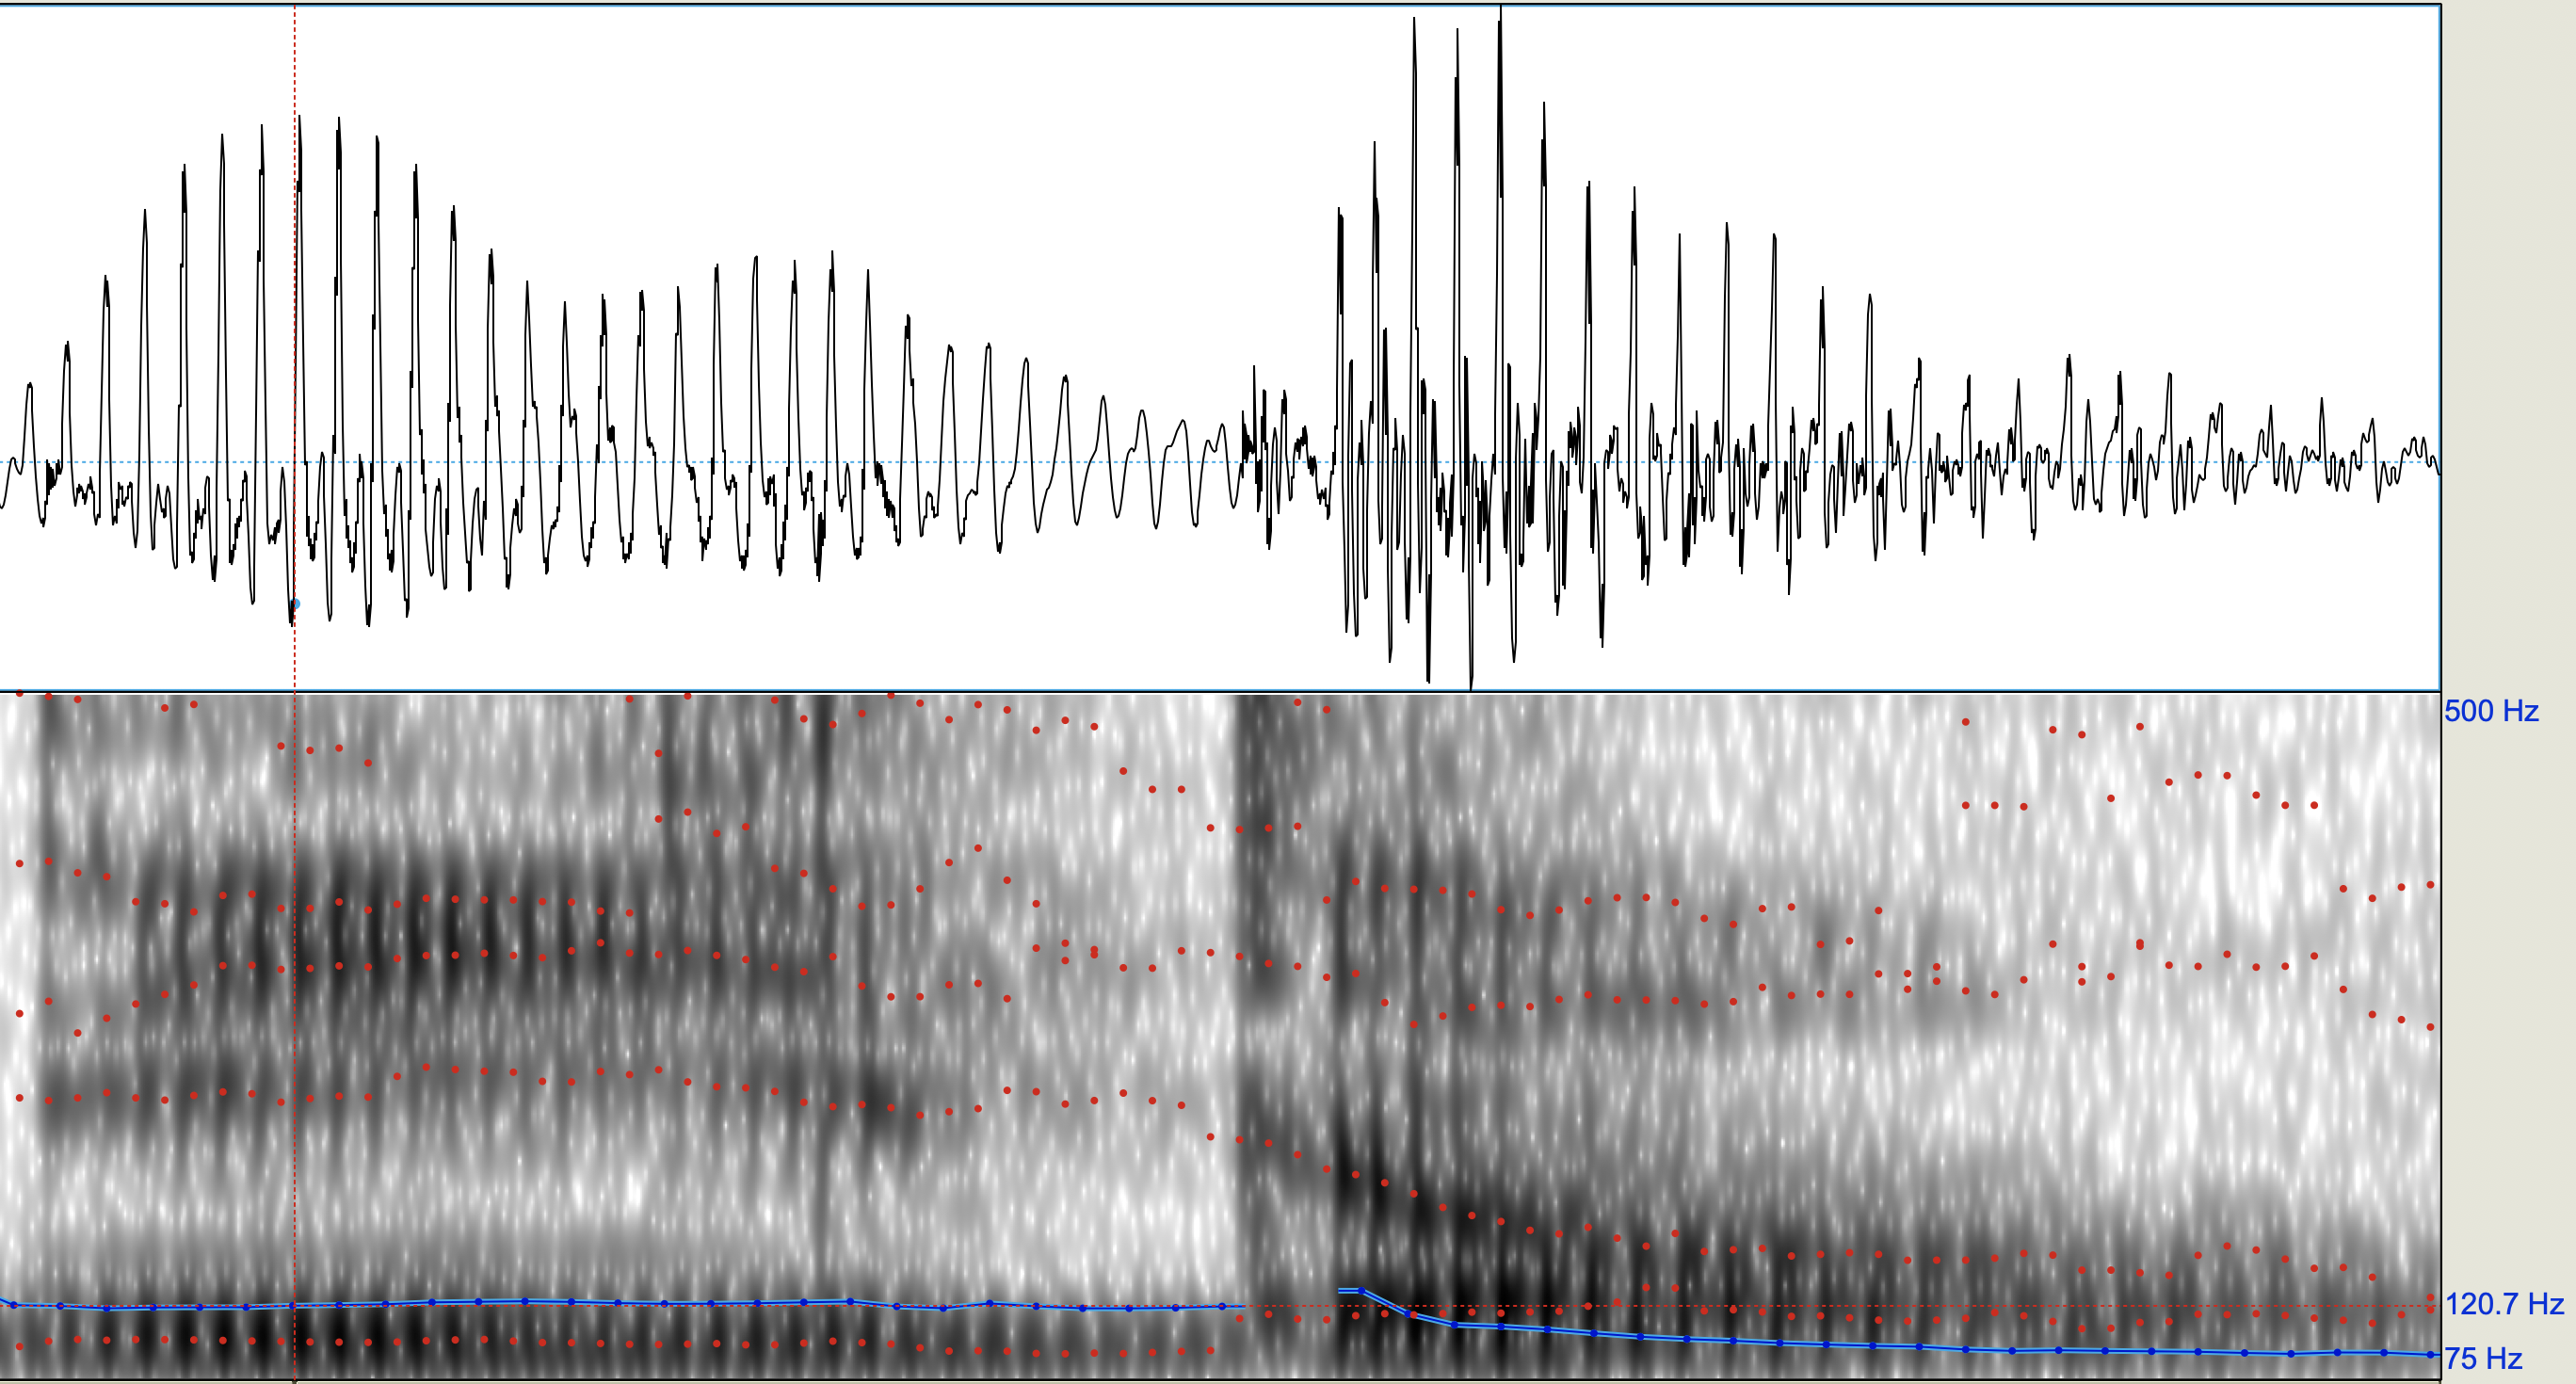
\includegraphics[scale=0.25]{imgs/nidou.png}
    \caption{Tone(51): [ni55 dou22]}
\end{figure}

The [dou22] in [ni55 dou22] sounds exactly like the fourth tone in Mandarin, mainly because it follows a high flat tone. The reason why I'm so sure about its auditory impression is that it sounds precisely the same as my last name. 

In conclusion, tones can be tricky enough when a syllable stands alone, and they can get even trickier when a syllable appears in consecutive speech. This study also makes me rethink tonal typology and how useful it can be for speech recognition of a tonal language. 

\end{document}